% **************************************************************************************************************
% A Classic Thesis Style
% An Homage to The Elements of Typographic Style
%
% Copyright (C) 2015 André Miede http://www.miede.de
%
% If you like the style then I would appreciate a postcard. My address 
% can be found in the file ClassicThesis.pdf. A collection of the 
% postcards I received so far is available online at 
% http://postcards.miede.de
%
% License:
% This program is free software; you can redistribute it and/or modify
% it under the terms of the GNU General Public License as published by
% the Free Software Foundation; either version 2 of the License, or
% (at your option) any later version.
%
% This program is distributed in the hope that it will be useful,
% but WITHOUT ANY WARRANTY; without even the implied warranty of
% MERCHANTABILITY or FITNESS FOR A PARTICULAR PURPOSE.  See the
% GNU General Public License for more details.
%
% You should have received a copy of the GNU General Public License
% along with this program; see the file COPYING.  If not, write to
% the Free Software Foundation, Inc., 59 Temple Place - Suite 330,
% Boston, MA 02111-1307, USA.
%
% **************************************************************************************************************
\RequirePackage{fix-cm} % fix some latex issues see: http://texdoc.net/texmf-dist/doc/latex/base/fixltx2e.pdf
\documentclass[ twoside,openright,titlepage,numbers=noenddot,headinclude,%1headlines,% letterpaper a4paper
                footinclude=true,cleardoublepage=empty,abstractoff, % <--- obsolete, remove (todo)
                BCOR=5mm,paper=a4,fontsize=11pt,%11pt,a4paper,%
                ngerman,american,%
                ]{scrreprt}

%********************************************************************
% Note: Make all your adjustments in here
%*******************************************************
% ****************************************************************************************************
% classicthesis-config.tex 
% formerly known as loadpackages.sty, classicthesis-ldpkg.sty, and classicthesis-preamble.sty 
% Use it at the beginning of your ClassicThesis.tex, or as a LaTeX Preamble 
% in your ClassicThesis.{tex,lyx} with % ****************************************************************************************************
% classicthesis-config.tex 
% formerly known as loadpackages.sty, classicthesis-ldpkg.sty, and classicthesis-preamble.sty 
% Use it at the beginning of your ClassicThesis.tex, or as a LaTeX Preamble 
% in your ClassicThesis.{tex,lyx} with % ****************************************************************************************************
% classicthesis-config.tex 
% formerly known as loadpackages.sty, classicthesis-ldpkg.sty, and classicthesis-preamble.sty 
% Use it at the beginning of your ClassicThesis.tex, or as a LaTeX Preamble 
% in your ClassicThesis.{tex,lyx} with \input{classicthesis-config}
% ****************************************************************************************************  
% If you like the classicthesis, then I would appreciate a postcard. 
% My address can be found in the file ClassicThesis.pdf. A collection 
% of the postcards I received so far is available online at 
% http://postcards.miede.de
% ****************************************************************************************************


% ****************************************************************************************************
% 0. Set the encoding of your files. UTF-8 is the only sensible encoding nowadays. If you can't read
% äöüßáéçèê∂åëæƒÏ€ then change the encoding setting in your editor, not the line below. If your editor
% does not support utf8 use another editor!
% ****************************************************************************************************
\PassOptionsToPackage{utf8}{inputenc}
    \usepackage{inputenc}

% ****************************************************************************************************
% 1. Configure classicthesis for your needs here, e.g., remove "drafting" below 
% in order to deactivate the time-stamp on the pages
% ****************************************************************************************************
\PassOptionsToPackage{eulerchapternumbers,listings,%drafting,%
                      pdfspacing,floatperchapter,%linedheaders,%
                      beramono,dottedtoc,%
                      subfig,eulermath,parts}{classicthesis}                                        
% ********************************************************************
% Available options for classicthesis.sty 
% (see ClassicThesis.pdf for more information):
% drafting
% parts nochapters linedheaders
% eulerchapternumbers beramono eulermath pdfspacing minionprospacing
% tocaligned dottedtoc manychapters
% listings floatperchapter subfig
% ********************************************************************


% ****************************************************************************************************
% 2. Personal data and user ad-hoc commands
% ****************************************************************************************************
\newcommand{\myTitle}{An Online Stream Processor for Timely Dataflow\xspace}
\newcommand{\myName}{Sebastian Wicki\xspace}
\newcommand{\myVersion}{version 0.1\xspace}

% ********************************************************************
% Setup, finetuning, and useful commands
% ********************************************************************
\newcounter{dummy} % necessary for correct hyperlinks (to index, bib, etc.)
\newlength{\abcd} % for ab..z string length calculation
\newcommand{\ie}{i.\,e.}
\newcommand{\Ie}{I.\,e.}
\newcommand{\eg}{e.\,g.}
\newcommand{\Eg}{E.\,g.} 
% ****************************************************************************************************


% ****************************************************************************************************
% 3. Loading some handy packages
% ****************************************************************************************************
% ********************************************************************
% Shut up warnings
% ********************************************************************
\usepackage{silence}
\WarningFilter{scrreprt}{Usage of package `titlesec'}
%\WarningFilter{scrreprt}{Activating an ugly workaround}
\WarningFilter{fixltx2e}{}
\WarningFilter{titlesec}{Non standard sectioning command detected}

% ******************************************************************** 
% Packages with options that might require adjustments
% ******************************************************************** 
%\PassOptionsToPackage{ngerman,american}{babel}   % change this to your language(s)
% Spanish languages need extra options in order to work with this template
%\PassOptionsToPackage{spanish,es-lcroman}{babel}
    \usepackage{babel}                  

\usepackage{hyphenat}
\hyphenation{que-ries data-flow time-stamp time-ly}

\newcommand\TODO[1]{%
\ifthenelse{\equal{#1}{}}%
{\textcolor{Maroon}{\textbf{TODO.}}}%
{{\color{Maroon} \bfseries TODO: #1}}%
}

\usepackage{verbatim}

\usepackage{csquotes}
\PassOptionsToPackage{%
    %backend=biber, %instead of bibtex
    backend=bibtex8,bibencoding=ascii,%
    language=auto,%
    style=numeric-comp,%
    %style=authoryear-comp, % Author 1999, 2010
    %bibstyle=authoryear,dashed=false, % dashed: substitute rep. author with ---
    sorting=nyt, % name, year, title
    maxbibnames=10, % default: 3, et al.
    %backref=true,%
    natbib=true % natbib compatibility mode (\citep and \citet still work)
}{biblatex}
    \usepackage{biblatex}

\PassOptionsToPackage{fleqn}{amsmath}       % math environments and more by the AMS 
    \usepackage{amsmath}

% ******************************************************************** 
% General useful packages
% ******************************************************************** 
\PassOptionsToPackage{T1}{fontenc} % T2A for cyrillics
    \usepackage{fontenc}     
\usepackage{textcomp} % fix warning with missing font shapes
\usepackage{scrhack} % fix warnings when using KOMA with listings package          
\usepackage{xspace} % to get the spacing after macros right  
\usepackage{mparhack} % get marginpar right
\usepackage{fixltx2e} % fixes some LaTeX stuff --> since 2015 in the LaTeX kernel (see below)
%\usepackage[latest]{latexrelease} % will be used once available in more distributions (ISSUE #107)
\PassOptionsToPackage{printonlyused,smaller}{acronym} 
    \usepackage{acronym} % nice macros for handling all acronyms in the thesis
    %\renewcommand{\bflabel}[1]{{#1}\hfill} % fix the list of acronyms --> no longer working
    %\renewcommand*{\acsfont}[1]{\textsc{#1}} 
    \renewcommand*{\aclabelfont}[1]{\acsfont{#1}}
% ****************************************************************************************************


% ****************************************************************************************************
% 4. Setup floats: tables, (sub)figures, and captions
% ****************************************************************************************************
\usepackage{tabularx} % better tables
    \setlength{\extrarowheight}{3pt} % increase table row height
\newcommand{\tableheadline}[1]{\multicolumn{1}{c}{\spacedlowsmallcaps{#1}}}
\newcommand{\myfloatalign}{\centering} % to be used with each float for alignment
\usepackage{caption}
% Thanks to cgnieder and Claus Lahiri
% http://tex.stackexchange.com/questions/69349/spacedlowsmallcaps-in-caption-label
% [REMOVED DUE TO OTHER PROBLEMS, SEE ISSUE #82]    
%\DeclareCaptionLabelFormat{smallcaps}{\bothIfFirst{#1}{~}\MakeTextLowercase{\textsc{#2}}}
%\captionsetup{font=small,labelformat=smallcaps} % format=hang,
\captionsetup{font=small,labelfont=it,format=plain} % format=hang,
\usepackage{subfig}  
% ****************************************************************************************************


% ****************************************************************************************************
% 5. Setup code listings
% ****************************************************************************************************
\usepackage{listings} 
%\lstset{emph={trueIndex,root},emphstyle=\color{BlueViolet}}%\underbar} % for special keywords

% Define Language
\lstdefinelanguage{Rust}
{
  % list of keywords
  morekeywords={
    abstract,alignof,as,become,box,break,const,continue,crate,do,else,enum,
        extern,false,final,fn,for,if,impl,in,let,loop,macro,match,mod,move,mut,
        offsetof,override,priv,proc,pub,pure,ref,return,Self,self,sizeof,
        static,struct,super,trait,true,type,typeof,unsafe,unsized,use,virtual,
        where,while,yield
  },
  otherkeywords={:,\.,|,=,=>,->,\#!,?},
  sensitive, % keywords are not case-sensitive
  morecomment=[l]{//}, % l is for line comment
  morecomment=[s]{/*}{*/}, % s is for start and end delimiter
  morestring=[b]" % defines that strings are enclosed in double quotes
}

\lstset{language=Rust,%C++,
    morekeywords={PassOptionsToPackage,selectlanguage},
    keywordstyle=\color{RoyalBlue},%\bfseries,
    basicstyle=\small\color{darkgray}\ttfamily,
    identifierstyle=\color{Black},
    commentstyle=\color{Green}\ttfamily,
    stringstyle=\color{Maroon}\ttfamily,
    numbers=none,%left,%
    numberstyle=\scriptsize,%\tiny
    stepnumber=5,
    numbersep=8pt,
    showstringspaces=false,
    breaklines=true,
    %frameround=tttt,
    frame=single,
    rulecolor=\color{lstbackground},
    backgroundcolor=\color{lstbackground},
    captionpos=b,
    belowcaptionskip=.75\baselineskip,
    aboveskip=\baselineskip,
} 
% ****************************************************************************************************             


% ****************************************************************************************************
% 6. PDFLaTeX, hyperreferences and citation backreferences
% ****************************************************************************************************
% ********************************************************************
% Using PDFLaTeX
% ********************************************************************
\PassOptionsToPackage{pdftex,hyperfootnotes=false,pdfpagelabels}{hyperref}
    \usepackage{hyperref}  % backref linktocpage pagebackref
\pdfcompresslevel=9
\pdfadjustspacing=1 
\PassOptionsToPackage{pdftex}{graphicx}
    \usepackage{graphicx} 
 

% ********************************************************************
% Hyperreferences
% ********************************************************************
\hypersetup{%
    %draft, % = no hyperlinking at all (useful in b/w printouts)
    colorlinks=true, linktocpage=true, pdfstartpage=3, pdfstartview=FitV,%
    % uncomment the following line if you want to have black links (e.g., for printing)
    %colorlinks=false, linktocpage=false, pdfstartpage=3, pdfstartview=FitV, pdfborder={0 0 0},%
    breaklinks=true, pdfpagemode=UseNone, pageanchor=true, pdfpagemode=UseOutlines,%
    plainpages=false, bookmarksnumbered, bookmarksopen=true, bookmarksopenlevel=1,%
    hypertexnames=true, pdfhighlight=/O,%nesting=true,%frenchlinks,%
    urlcolor=webbrown, linkcolor=RoyalBlue, citecolor=webgreen, %pagecolor=RoyalBlue,%
    %urlcolor=Black, linkcolor=Black, citecolor=Black, %pagecolor=Black,%
    pdftitle={\myTitle},%
    pdfauthor={\textcopyright\ Sebastian Wicki, Systems Group, Department of Computer Science, ETH Zürich},%
    pdfsubject={},%
    pdfkeywords={},%
    pdfcreator={pdfLaTeX},%
    pdfproducer={LaTeX with hyperref and classicthesis}%
}   

% ********************************************************************
% Setup autoreferences
% ********************************************************************
% There are some issues regarding autorefnames
% http://www.ureader.de/msg/136221647.aspx
% http://www.tex.ac.uk/cgi-bin/texfaq2html?label=latexwords
% you have to redefine the makros for the 
% language you use, e.g., american, ngerman
% (as chosen when loading babel/AtBeginDocument)
% ********************************************************************
\makeatletter
\@ifpackageloaded{babel}%
    {%
       \addto\extrasamerican{%
			\renewcommand*{\figureautorefname}{Figure}%
			\renewcommand*{\tableautorefname}{Table}%
			\renewcommand*{\partautorefname}{Part}%
			\renewcommand*{\chapterautorefname}{Chapter}%
			\renewcommand*{\sectionautorefname}{Section}%
			\renewcommand*{\subsectionautorefname}{Section}%
			\renewcommand*{\subsubsectionautorefname}{Section}%     
                }%
       \addto\extrasngerman{% 
			\renewcommand*{\paragraphautorefname}{Absatz}%
			\renewcommand*{\subparagraphautorefname}{Unterabsatz}%
			\renewcommand*{\footnoteautorefname}{Fu\"snote}%
			\renewcommand*{\FancyVerbLineautorefname}{Zeile}%
			\renewcommand*{\theoremautorefname}{Theorem}%
			\renewcommand*{\appendixautorefname}{Anhang}%
			\renewcommand*{\equationautorefname}{Gleichung}%        
			\renewcommand*{\itemautorefname}{Punkt}%
                }%  
            % Fix to getting autorefs for subfigures right (thanks to Belinda Vogt for changing the definition)
            \providecommand{\subfigureautorefname}{\figureautorefname}%             
    }{\relax}
\makeatother


% ****************************************************************************************************
% 7. Last calls before the bar closes
% ****************************************************************************************************
% ********************************************************************
% Development Stuff
% ********************************************************************
%\listfiles
%\PassOptionsToPackage{l2tabu,orthodox,abort}{nag}
%   \usepackage{nag}
%\PassOptionsToPackage{warning, all}{onlyamsmath}
%   \usepackage{onlyamsmath}

% ********************************************************************
% Last, but not least...
% ********************************************************************
\usepackage{classicthesis} 
% ****************************************************************************************************

% ****************************************************************************************************
% 8. Further adjustments (experimental)
% ****************************************************************************************************
% ********************************************************************
% Changing the text area
% ********************************************************************
%\linespread{1.05} % a bit more for Palatino
%\areaset[current]{312pt}{761pt} % 686 (factor 2.2) + 33 head + 42 head \the\footskip
%\setlength{\marginparwidth}{7em}%
%\setlength{\marginparsep}{2em}%

% ********************************************************************
% Using different fonts
% ********************************************************************
%\usepackage[oldstylenums]{kpfonts} % oldstyle notextcomp
%\usepackage[osf]{libertine}
%\usepackage[light,condensed,math]{iwona}
%\renewcommand{\sfdefault}{iwona}
%\usepackage{lmodern} % <-- no osf support :-(
%\usepackage{cfr-lm} % 
%\usepackage[urw-garamond]{mathdesign} <-- no osf support :-(
%\usepackage[default,osfigures]{opensans} % scale=0.95 
%\usepackage[sfdefault]{FiraSans}
% ****************************************************************************************************

% ********************************************************************
% Systems Group title page
% ********************************************************************
\usepackage[masterthesis]{systems-cover/systems-cover}
\covernum{155}
\covertitle{\myTitle}
\coverauthor{\myName}
\coversupervisedby{Dr.\ Desislava Dimitrova \\ Dr.\ John Liagouris \\ Prof.\ Timothy Roscoe}
\coverdate{May 2016 -- November 2016}

% ********************************************************************
% For the Declaration of Originality
% ********************************************************************
\usepackage{pdfpages}

% ****************************************************************************************************  
% If you like the classicthesis, then I would appreciate a postcard. 
% My address can be found in the file ClassicThesis.pdf. A collection 
% of the postcards I received so far is available online at 
% http://postcards.miede.de
% ****************************************************************************************************


% ****************************************************************************************************
% 0. Set the encoding of your files. UTF-8 is the only sensible encoding nowadays. If you can't read
% äöüßáéçèê∂åëæƒÏ€ then change the encoding setting in your editor, not the line below. If your editor
% does not support utf8 use another editor!
% ****************************************************************************************************
\PassOptionsToPackage{utf8}{inputenc}
    \usepackage{inputenc}

% ****************************************************************************************************
% 1. Configure classicthesis for your needs here, e.g., remove "drafting" below 
% in order to deactivate the time-stamp on the pages
% ****************************************************************************************************
\PassOptionsToPackage{eulerchapternumbers,listings,%drafting,%
                      pdfspacing,floatperchapter,%linedheaders,%
                      beramono,dottedtoc,%
                      subfig,eulermath,parts}{classicthesis}                                        
% ********************************************************************
% Available options for classicthesis.sty 
% (see ClassicThesis.pdf for more information):
% drafting
% parts nochapters linedheaders
% eulerchapternumbers beramono eulermath pdfspacing minionprospacing
% tocaligned dottedtoc manychapters
% listings floatperchapter subfig
% ********************************************************************


% ****************************************************************************************************
% 2. Personal data and user ad-hoc commands
% ****************************************************************************************************
\newcommand{\myTitle}{An Online Stream Processor for Timely Dataflow\xspace}
\newcommand{\myName}{Sebastian Wicki\xspace}
\newcommand{\myVersion}{version 0.1\xspace}

% ********************************************************************
% Setup, finetuning, and useful commands
% ********************************************************************
\newcounter{dummy} % necessary for correct hyperlinks (to index, bib, etc.)
\newlength{\abcd} % for ab..z string length calculation
\newcommand{\ie}{i.\,e.}
\newcommand{\Ie}{I.\,e.}
\newcommand{\eg}{e.\,g.}
\newcommand{\Eg}{E.\,g.} 
% ****************************************************************************************************


% ****************************************************************************************************
% 3. Loading some handy packages
% ****************************************************************************************************
% ********************************************************************
% Shut up warnings
% ********************************************************************
\usepackage{silence}
\WarningFilter{scrreprt}{Usage of package `titlesec'}
%\WarningFilter{scrreprt}{Activating an ugly workaround}
\WarningFilter{fixltx2e}{}
\WarningFilter{titlesec}{Non standard sectioning command detected}

% ******************************************************************** 
% Packages with options that might require adjustments
% ******************************************************************** 
%\PassOptionsToPackage{ngerman,american}{babel}   % change this to your language(s)
% Spanish languages need extra options in order to work with this template
%\PassOptionsToPackage{spanish,es-lcroman}{babel}
    \usepackage{babel}                  

\usepackage{hyphenat}
\hyphenation{que-ries data-flow time-stamp time-ly}

\newcommand\TODO[1]{%
\ifthenelse{\equal{#1}{}}%
{\textcolor{Maroon}{\textbf{TODO.}}}%
{{\color{Maroon} \bfseries TODO: #1}}%
}

\usepackage{verbatim}

\usepackage{csquotes}
\PassOptionsToPackage{%
    %backend=biber, %instead of bibtex
    backend=bibtex8,bibencoding=ascii,%
    language=auto,%
    style=numeric-comp,%
    %style=authoryear-comp, % Author 1999, 2010
    %bibstyle=authoryear,dashed=false, % dashed: substitute rep. author with ---
    sorting=nyt, % name, year, title
    maxbibnames=10, % default: 3, et al.
    %backref=true,%
    natbib=true % natbib compatibility mode (\citep and \citet still work)
}{biblatex}
    \usepackage{biblatex}

\PassOptionsToPackage{fleqn}{amsmath}       % math environments and more by the AMS 
    \usepackage{amsmath}

% ******************************************************************** 
% General useful packages
% ******************************************************************** 
\PassOptionsToPackage{T1}{fontenc} % T2A for cyrillics
    \usepackage{fontenc}     
\usepackage{textcomp} % fix warning with missing font shapes
\usepackage{scrhack} % fix warnings when using KOMA with listings package          
\usepackage{xspace} % to get the spacing after macros right  
\usepackage{mparhack} % get marginpar right
\usepackage{fixltx2e} % fixes some LaTeX stuff --> since 2015 in the LaTeX kernel (see below)
%\usepackage[latest]{latexrelease} % will be used once available in more distributions (ISSUE #107)
\PassOptionsToPackage{printonlyused,smaller}{acronym} 
    \usepackage{acronym} % nice macros for handling all acronyms in the thesis
    %\renewcommand{\bflabel}[1]{{#1}\hfill} % fix the list of acronyms --> no longer working
    %\renewcommand*{\acsfont}[1]{\textsc{#1}} 
    \renewcommand*{\aclabelfont}[1]{\acsfont{#1}}
% ****************************************************************************************************


% ****************************************************************************************************
% 4. Setup floats: tables, (sub)figures, and captions
% ****************************************************************************************************
\usepackage{tabularx} % better tables
    \setlength{\extrarowheight}{3pt} % increase table row height
\newcommand{\tableheadline}[1]{\multicolumn{1}{c}{\spacedlowsmallcaps{#1}}}
\newcommand{\myfloatalign}{\centering} % to be used with each float for alignment
\usepackage{caption}
% Thanks to cgnieder and Claus Lahiri
% http://tex.stackexchange.com/questions/69349/spacedlowsmallcaps-in-caption-label
% [REMOVED DUE TO OTHER PROBLEMS, SEE ISSUE #82]    
%\DeclareCaptionLabelFormat{smallcaps}{\bothIfFirst{#1}{~}\MakeTextLowercase{\textsc{#2}}}
%\captionsetup{font=small,labelformat=smallcaps} % format=hang,
\captionsetup{font=small,labelfont=it,format=plain} % format=hang,
\usepackage{subfig}  
% ****************************************************************************************************


% ****************************************************************************************************
% 5. Setup code listings
% ****************************************************************************************************
\usepackage{listings} 
%\lstset{emph={trueIndex,root},emphstyle=\color{BlueViolet}}%\underbar} % for special keywords

% Define Language
\lstdefinelanguage{Rust}
{
  % list of keywords
  morekeywords={
    abstract,alignof,as,become,box,break,const,continue,crate,do,else,enum,
        extern,false,final,fn,for,if,impl,in,let,loop,macro,match,mod,move,mut,
        offsetof,override,priv,proc,pub,pure,ref,return,Self,self,sizeof,
        static,struct,super,trait,true,type,typeof,unsafe,unsized,use,virtual,
        where,while,yield
  },
  otherkeywords={:,\.,|,=,=>,->,\#!,?},
  sensitive, % keywords are not case-sensitive
  morecomment=[l]{//}, % l is for line comment
  morecomment=[s]{/*}{*/}, % s is for start and end delimiter
  morestring=[b]" % defines that strings are enclosed in double quotes
}

\lstset{language=Rust,%C++,
    morekeywords={PassOptionsToPackage,selectlanguage},
    keywordstyle=\color{RoyalBlue},%\bfseries,
    basicstyle=\small\color{darkgray}\ttfamily,
    identifierstyle=\color{Black},
    commentstyle=\color{Green}\ttfamily,
    stringstyle=\color{Maroon}\ttfamily,
    numbers=none,%left,%
    numberstyle=\scriptsize,%\tiny
    stepnumber=5,
    numbersep=8pt,
    showstringspaces=false,
    breaklines=true,
    %frameround=tttt,
    frame=single,
    rulecolor=\color{lstbackground},
    backgroundcolor=\color{lstbackground},
    captionpos=b,
    belowcaptionskip=.75\baselineskip,
    aboveskip=\baselineskip,
} 
% ****************************************************************************************************             


% ****************************************************************************************************
% 6. PDFLaTeX, hyperreferences and citation backreferences
% ****************************************************************************************************
% ********************************************************************
% Using PDFLaTeX
% ********************************************************************
\PassOptionsToPackage{pdftex,hyperfootnotes=false,pdfpagelabels}{hyperref}
    \usepackage{hyperref}  % backref linktocpage pagebackref
\pdfcompresslevel=9
\pdfadjustspacing=1 
\PassOptionsToPackage{pdftex}{graphicx}
    \usepackage{graphicx} 
 

% ********************************************************************
% Hyperreferences
% ********************************************************************
\hypersetup{%
    %draft, % = no hyperlinking at all (useful in b/w printouts)
    colorlinks=true, linktocpage=true, pdfstartpage=3, pdfstartview=FitV,%
    % uncomment the following line if you want to have black links (e.g., for printing)
    %colorlinks=false, linktocpage=false, pdfstartpage=3, pdfstartview=FitV, pdfborder={0 0 0},%
    breaklinks=true, pdfpagemode=UseNone, pageanchor=true, pdfpagemode=UseOutlines,%
    plainpages=false, bookmarksnumbered, bookmarksopen=true, bookmarksopenlevel=1,%
    hypertexnames=true, pdfhighlight=/O,%nesting=true,%frenchlinks,%
    urlcolor=webbrown, linkcolor=RoyalBlue, citecolor=webgreen, %pagecolor=RoyalBlue,%
    %urlcolor=Black, linkcolor=Black, citecolor=Black, %pagecolor=Black,%
    pdftitle={\myTitle},%
    pdfauthor={\textcopyright\ Sebastian Wicki, Systems Group, Department of Computer Science, ETH Zürich},%
    pdfsubject={},%
    pdfkeywords={},%
    pdfcreator={pdfLaTeX},%
    pdfproducer={LaTeX with hyperref and classicthesis}%
}   

% ********************************************************************
% Setup autoreferences
% ********************************************************************
% There are some issues regarding autorefnames
% http://www.ureader.de/msg/136221647.aspx
% http://www.tex.ac.uk/cgi-bin/texfaq2html?label=latexwords
% you have to redefine the makros for the 
% language you use, e.g., american, ngerman
% (as chosen when loading babel/AtBeginDocument)
% ********************************************************************
\makeatletter
\@ifpackageloaded{babel}%
    {%
       \addto\extrasamerican{%
			\renewcommand*{\figureautorefname}{Figure}%
			\renewcommand*{\tableautorefname}{Table}%
			\renewcommand*{\partautorefname}{Part}%
			\renewcommand*{\chapterautorefname}{Chapter}%
			\renewcommand*{\sectionautorefname}{Section}%
			\renewcommand*{\subsectionautorefname}{Section}%
			\renewcommand*{\subsubsectionautorefname}{Section}%     
                }%
       \addto\extrasngerman{% 
			\renewcommand*{\paragraphautorefname}{Absatz}%
			\renewcommand*{\subparagraphautorefname}{Unterabsatz}%
			\renewcommand*{\footnoteautorefname}{Fu\"snote}%
			\renewcommand*{\FancyVerbLineautorefname}{Zeile}%
			\renewcommand*{\theoremautorefname}{Theorem}%
			\renewcommand*{\appendixautorefname}{Anhang}%
			\renewcommand*{\equationautorefname}{Gleichung}%        
			\renewcommand*{\itemautorefname}{Punkt}%
                }%  
            % Fix to getting autorefs for subfigures right (thanks to Belinda Vogt for changing the definition)
            \providecommand{\subfigureautorefname}{\figureautorefname}%             
    }{\relax}
\makeatother


% ****************************************************************************************************
% 7. Last calls before the bar closes
% ****************************************************************************************************
% ********************************************************************
% Development Stuff
% ********************************************************************
%\listfiles
%\PassOptionsToPackage{l2tabu,orthodox,abort}{nag}
%   \usepackage{nag}
%\PassOptionsToPackage{warning, all}{onlyamsmath}
%   \usepackage{onlyamsmath}

% ********************************************************************
% Last, but not least...
% ********************************************************************
\usepackage{classicthesis} 
% ****************************************************************************************************

% ****************************************************************************************************
% 8. Further adjustments (experimental)
% ****************************************************************************************************
% ********************************************************************
% Changing the text area
% ********************************************************************
%\linespread{1.05} % a bit more for Palatino
%\areaset[current]{312pt}{761pt} % 686 (factor 2.2) + 33 head + 42 head \the\footskip
%\setlength{\marginparwidth}{7em}%
%\setlength{\marginparsep}{2em}%

% ********************************************************************
% Using different fonts
% ********************************************************************
%\usepackage[oldstylenums]{kpfonts} % oldstyle notextcomp
%\usepackage[osf]{libertine}
%\usepackage[light,condensed,math]{iwona}
%\renewcommand{\sfdefault}{iwona}
%\usepackage{lmodern} % <-- no osf support :-(
%\usepackage{cfr-lm} % 
%\usepackage[urw-garamond]{mathdesign} <-- no osf support :-(
%\usepackage[default,osfigures]{opensans} % scale=0.95 
%\usepackage[sfdefault]{FiraSans}
% ****************************************************************************************************

% ********************************************************************
% Systems Group title page
% ********************************************************************
\usepackage[masterthesis]{systems-cover/systems-cover}
\covernum{155}
\covertitle{\myTitle}
\coverauthor{\myName}
\coversupervisedby{Dr.\ Desislava Dimitrova \\ Dr.\ John Liagouris \\ Prof.\ Timothy Roscoe}
\coverdate{May 2016 -- November 2016}

% ********************************************************************
% For the Declaration of Originality
% ********************************************************************
\usepackage{pdfpages}

% ****************************************************************************************************  
% If you like the classicthesis, then I would appreciate a postcard. 
% My address can be found in the file ClassicThesis.pdf. A collection 
% of the postcards I received so far is available online at 
% http://postcards.miede.de
% ****************************************************************************************************


% ****************************************************************************************************
% 0. Set the encoding of your files. UTF-8 is the only sensible encoding nowadays. If you can't read
% äöüßáéçèê∂åëæƒÏ€ then change the encoding setting in your editor, not the line below. If your editor
% does not support utf8 use another editor!
% ****************************************************************************************************
\PassOptionsToPackage{utf8}{inputenc}
    \usepackage{inputenc}

% ****************************************************************************************************
% 1. Configure classicthesis for your needs here, e.g., remove "drafting" below 
% in order to deactivate the time-stamp on the pages
% ****************************************************************************************************
\PassOptionsToPackage{eulerchapternumbers,listings,%drafting,%
                      pdfspacing,floatperchapter,%linedheaders,%
                      beramono,dottedtoc,%
                      subfig,eulermath,parts}{classicthesis}                                        
% ********************************************************************
% Available options for classicthesis.sty 
% (see ClassicThesis.pdf for more information):
% drafting
% parts nochapters linedheaders
% eulerchapternumbers beramono eulermath pdfspacing minionprospacing
% tocaligned dottedtoc manychapters
% listings floatperchapter subfig
% ********************************************************************


% ****************************************************************************************************
% 2. Personal data and user ad-hoc commands
% ****************************************************************************************************
\newcommand{\myTitle}{An Online Stream Processor for Timely Dataflow\xspace}
\newcommand{\myName}{Sebastian Wicki\xspace}
\newcommand{\myVersion}{version 0.1\xspace}

% ********************************************************************
% Setup, finetuning, and useful commands
% ********************************************************************
\newcounter{dummy} % necessary for correct hyperlinks (to index, bib, etc.)
\newlength{\abcd} % for ab..z string length calculation
\newcommand{\ie}{i.\,e.}
\newcommand{\Ie}{I.\,e.}
\newcommand{\eg}{e.\,g.}
\newcommand{\Eg}{E.\,g.} 
% ****************************************************************************************************


% ****************************************************************************************************
% 3. Loading some handy packages
% ****************************************************************************************************
% ********************************************************************
% Shut up warnings
% ********************************************************************
\usepackage{silence}
\WarningFilter{scrreprt}{Usage of package `titlesec'}
%\WarningFilter{scrreprt}{Activating an ugly workaround}
\WarningFilter{fixltx2e}{}
\WarningFilter{titlesec}{Non standard sectioning command detected}

% ******************************************************************** 
% Packages with options that might require adjustments
% ******************************************************************** 
%\PassOptionsToPackage{ngerman,american}{babel}   % change this to your language(s)
% Spanish languages need extra options in order to work with this template
%\PassOptionsToPackage{spanish,es-lcroman}{babel}
    \usepackage{babel}                  

\usepackage{hyphenat}
\hyphenation{que-ries data-flow time-stamp time-ly}

\newcommand\TODO[1]{%
\ifthenelse{\equal{#1}{}}%
{\textcolor{Maroon}{\textbf{TODO.}}}%
{{\color{Maroon} \bfseries TODO: #1}}%
}

\usepackage{verbatim}

\usepackage{csquotes}
\PassOptionsToPackage{%
    %backend=biber, %instead of bibtex
    backend=bibtex8,bibencoding=ascii,%
    language=auto,%
    style=numeric-comp,%
    %style=authoryear-comp, % Author 1999, 2010
    %bibstyle=authoryear,dashed=false, % dashed: substitute rep. author with ---
    sorting=nyt, % name, year, title
    maxbibnames=10, % default: 3, et al.
    %backref=true,%
    natbib=true % natbib compatibility mode (\citep and \citet still work)
}{biblatex}
    \usepackage{biblatex}

\PassOptionsToPackage{fleqn}{amsmath}       % math environments and more by the AMS 
    \usepackage{amsmath}

% ******************************************************************** 
% General useful packages
% ******************************************************************** 
\PassOptionsToPackage{T1}{fontenc} % T2A for cyrillics
    \usepackage{fontenc}     
\usepackage{textcomp} % fix warning with missing font shapes
\usepackage{scrhack} % fix warnings when using KOMA with listings package          
\usepackage{xspace} % to get the spacing after macros right  
\usepackage{mparhack} % get marginpar right
\usepackage{fixltx2e} % fixes some LaTeX stuff --> since 2015 in the LaTeX kernel (see below)
%\usepackage[latest]{latexrelease} % will be used once available in more distributions (ISSUE #107)
\PassOptionsToPackage{printonlyused,smaller}{acronym} 
    \usepackage{acronym} % nice macros for handling all acronyms in the thesis
    %\renewcommand{\bflabel}[1]{{#1}\hfill} % fix the list of acronyms --> no longer working
    %\renewcommand*{\acsfont}[1]{\textsc{#1}} 
    \renewcommand*{\aclabelfont}[1]{\acsfont{#1}}
% ****************************************************************************************************


% ****************************************************************************************************
% 4. Setup floats: tables, (sub)figures, and captions
% ****************************************************************************************************
\usepackage{tabularx} % better tables
    \setlength{\extrarowheight}{3pt} % increase table row height
\newcommand{\tableheadline}[1]{\multicolumn{1}{c}{\spacedlowsmallcaps{#1}}}
\newcommand{\myfloatalign}{\centering} % to be used with each float for alignment
\usepackage{caption}
% Thanks to cgnieder and Claus Lahiri
% http://tex.stackexchange.com/questions/69349/spacedlowsmallcaps-in-caption-label
% [REMOVED DUE TO OTHER PROBLEMS, SEE ISSUE #82]    
%\DeclareCaptionLabelFormat{smallcaps}{\bothIfFirst{#1}{~}\MakeTextLowercase{\textsc{#2}}}
%\captionsetup{font=small,labelformat=smallcaps} % format=hang,
\captionsetup{font=small,labelfont=it,format=plain} % format=hang,
\usepackage{subfig}  
% ****************************************************************************************************


% ****************************************************************************************************
% 5. Setup code listings
% ****************************************************************************************************
\usepackage{listings} 
%\lstset{emph={trueIndex,root},emphstyle=\color{BlueViolet}}%\underbar} % for special keywords

% Define Language
\lstdefinelanguage{Rust}
{
  % list of keywords
  morekeywords={
    abstract,alignof,as,become,box,break,const,continue,crate,do,else,enum,
        extern,false,final,fn,for,if,impl,in,let,loop,macro,match,mod,move,mut,
        offsetof,override,priv,proc,pub,pure,ref,return,Self,self,sizeof,
        static,struct,super,trait,true,type,typeof,unsafe,unsized,use,virtual,
        where,while,yield
  },
  otherkeywords={:,\.,|,=,=>,->,\#!,?},
  sensitive, % keywords are not case-sensitive
  morecomment=[l]{//}, % l is for line comment
  morecomment=[s]{/*}{*/}, % s is for start and end delimiter
  morestring=[b]" % defines that strings are enclosed in double quotes
}

\lstset{language=Rust,%C++,
    morekeywords={PassOptionsToPackage,selectlanguage},
    keywordstyle=\color{RoyalBlue},%\bfseries,
    basicstyle=\small\color{darkgray}\ttfamily,
    identifierstyle=\color{Black},
    commentstyle=\color{Green}\ttfamily,
    stringstyle=\color{Maroon}\ttfamily,
    numbers=none,%left,%
    numberstyle=\scriptsize,%\tiny
    stepnumber=5,
    numbersep=8pt,
    showstringspaces=false,
    breaklines=true,
    %frameround=tttt,
    frame=single,
    rulecolor=\color{lstbackground},
    backgroundcolor=\color{lstbackground},
    captionpos=b,
    belowcaptionskip=.75\baselineskip,
    aboveskip=\baselineskip,
} 
% ****************************************************************************************************             


% ****************************************************************************************************
% 6. PDFLaTeX, hyperreferences and citation backreferences
% ****************************************************************************************************
% ********************************************************************
% Using PDFLaTeX
% ********************************************************************
\PassOptionsToPackage{pdftex,hyperfootnotes=false,pdfpagelabels}{hyperref}
    \usepackage{hyperref}  % backref linktocpage pagebackref
\pdfcompresslevel=9
\pdfadjustspacing=1 
\PassOptionsToPackage{pdftex}{graphicx}
    \usepackage{graphicx} 
 

% ********************************************************************
% Hyperreferences
% ********************************************************************
\hypersetup{%
    %draft, % = no hyperlinking at all (useful in b/w printouts)
    colorlinks=true, linktocpage=true, pdfstartpage=3, pdfstartview=FitV,%
    % uncomment the following line if you want to have black links (e.g., for printing)
    %colorlinks=false, linktocpage=false, pdfstartpage=3, pdfstartview=FitV, pdfborder={0 0 0},%
    breaklinks=true, pdfpagemode=UseNone, pageanchor=true, pdfpagemode=UseOutlines,%
    plainpages=false, bookmarksnumbered, bookmarksopen=true, bookmarksopenlevel=1,%
    hypertexnames=true, pdfhighlight=/O,%nesting=true,%frenchlinks,%
    urlcolor=webbrown, linkcolor=RoyalBlue, citecolor=webgreen, %pagecolor=RoyalBlue,%
    %urlcolor=Black, linkcolor=Black, citecolor=Black, %pagecolor=Black,%
    pdftitle={\myTitle},%
    pdfauthor={\textcopyright\ Sebastian Wicki, Systems Group, Department of Computer Science, ETH Zürich},%
    pdfsubject={},%
    pdfkeywords={},%
    pdfcreator={pdfLaTeX},%
    pdfproducer={LaTeX with hyperref and classicthesis}%
}   

% ********************************************************************
% Setup autoreferences
% ********************************************************************
% There are some issues regarding autorefnames
% http://www.ureader.de/msg/136221647.aspx
% http://www.tex.ac.uk/cgi-bin/texfaq2html?label=latexwords
% you have to redefine the makros for the 
% language you use, e.g., american, ngerman
% (as chosen when loading babel/AtBeginDocument)
% ********************************************************************
\makeatletter
\@ifpackageloaded{babel}%
    {%
       \addto\extrasamerican{%
			\renewcommand*{\figureautorefname}{Figure}%
			\renewcommand*{\tableautorefname}{Table}%
			\renewcommand*{\partautorefname}{Part}%
			\renewcommand*{\chapterautorefname}{Chapter}%
			\renewcommand*{\sectionautorefname}{Section}%
			\renewcommand*{\subsectionautorefname}{Section}%
			\renewcommand*{\subsubsectionautorefname}{Section}%     
                }%
       \addto\extrasngerman{% 
			\renewcommand*{\paragraphautorefname}{Absatz}%
			\renewcommand*{\subparagraphautorefname}{Unterabsatz}%
			\renewcommand*{\footnoteautorefname}{Fu\"snote}%
			\renewcommand*{\FancyVerbLineautorefname}{Zeile}%
			\renewcommand*{\theoremautorefname}{Theorem}%
			\renewcommand*{\appendixautorefname}{Anhang}%
			\renewcommand*{\equationautorefname}{Gleichung}%        
			\renewcommand*{\itemautorefname}{Punkt}%
                }%  
            % Fix to getting autorefs for subfigures right (thanks to Belinda Vogt for changing the definition)
            \providecommand{\subfigureautorefname}{\figureautorefname}%             
    }{\relax}
\makeatother


% ****************************************************************************************************
% 7. Last calls before the bar closes
% ****************************************************************************************************
% ********************************************************************
% Development Stuff
% ********************************************************************
%\listfiles
%\PassOptionsToPackage{l2tabu,orthodox,abort}{nag}
%   \usepackage{nag}
%\PassOptionsToPackage{warning, all}{onlyamsmath}
%   \usepackage{onlyamsmath}

% ********************************************************************
% Last, but not least...
% ********************************************************************
\usepackage{classicthesis} 
% ****************************************************************************************************

% ****************************************************************************************************
% 8. Further adjustments (experimental)
% ****************************************************************************************************
% ********************************************************************
% Changing the text area
% ********************************************************************
%\linespread{1.05} % a bit more for Palatino
%\areaset[current]{312pt}{761pt} % 686 (factor 2.2) + 33 head + 42 head \the\footskip
%\setlength{\marginparwidth}{7em}%
%\setlength{\marginparsep}{2em}%

% ********************************************************************
% Using different fonts
% ********************************************************************
%\usepackage[oldstylenums]{kpfonts} % oldstyle notextcomp
%\usepackage[osf]{libertine}
%\usepackage[light,condensed,math]{iwona}
%\renewcommand{\sfdefault}{iwona}
%\usepackage{lmodern} % <-- no osf support :-(
%\usepackage{cfr-lm} % 
%\usepackage[urw-garamond]{mathdesign} <-- no osf support :-(
%\usepackage[default,osfigures]{opensans} % scale=0.95 
%\usepackage[sfdefault]{FiraSans}
% ****************************************************************************************************

% ********************************************************************
% Systems Group title page
% ********************************************************************
\usepackage[masterthesis]{systems-cover/systems-cover}
\covernum{155}
\covertitle{\myTitle}
\coverauthor{\myName}
\coversupervisedby{Dr.\ Desislava Dimitrova \\ Dr.\ John Liagouris \\ Prof.\ Timothy Roscoe}
\coverdate{May 2016 -- November 2016}

% ********************************************************************
% For the Declaration of Originality
% ********************************************************************
\usepackage{pdfpages}


%********************************************************************
% Bibliographies
%*******************************************************
\addbibresource{bibliography.bib}

%********************************************************************
% Hyphenation
%*******************************************************
%\hyphenation{put special hyphenation here}

% ********************************************************************
% GO!GO!GO! MOVE IT!
%*******************************************************
\begin{document}
\frenchspacing
\raggedbottom
\selectlanguage{american} % american ngerman
%\renewcommand*{\bibname}{new name}
%\setbibpreamble{}
\pagenumbering{roman}
\pagestyle{plain}
%********************************************************************
% Frontmatter
%*******************************************************
% TODO \cleardoublepage%*******************************************************
% Abstract
%*******************************************************
%\renewcommand{\abstractname}{Abstract}
\pdfbookmark[1]{Abstract}{Abstract}
\begingroup
\let\clearpage\relax
\let\cleardoublepage\relax
\let\cleardoublepage\relax

\chapter*{Abstract}

Processing of unbounded data streams is increasingly important in many
applications. 

In this thesis we present a system for managing Timely Dataflow programs,


We demonstrate 

\endgroup

% TODO \cleardoublepage%*******************************************************
% Acknowledgments
%*******************************************************
\pdfbookmark[1]{Acknowledgments}{acknowledgments}

\begingroup
\chapter*{Acknowledgments}

I would like to thank Prof. Timothy Roscoe, not only for providing me with the
opportunity to work on this project, but also for his guidance along the way.

My thanks also goes to my supervisors, Dr. Desislava Dimitrova and Dr. John Liagouris.
This work would not have been possible without their great support and invaluable feedback.

Finally I would like to thank Andrea Lattuada and Zaheer Chothia, as their
initial inputs have gained me a better understanding of the particularities
of Timely Dataflow.

\endgroup

\pagestyle{scrheadings}
\cleardoublepage%*******************************************************
% Table of Contents
%*******************************************************
%\phantomsection
\refstepcounter{dummy}
\pdfbookmark[1]{\contentsname}{tableofcontents}
\setcounter{tocdepth}{2} % <-- 2 includes up to subsections in the ToC
\setcounter{secnumdepth}{3} % <-- 3 numbers up to subsubsections
\manualmark
\markboth{\spacedlowsmallcaps{\contentsname}}{\spacedlowsmallcaps{\contentsname}}
\tableofcontents 
\automark[section]{chapter}
\renewcommand{\chaptermark}[1]{\markboth{\spacedlowsmallcaps{#1}}{\spacedlowsmallcaps{#1}}}
\renewcommand{\sectionmark}[1]{\markright{\thesection\enspace\spacedlowsmallcaps{#1}}}
%*******************************************************
% List of Figures and of the Tables
%*******************************************************
\clearpage

\begingroup 
    \let\clearpage\relax
    \let\cleardoublepage\relax
    \let\cleardoublepage\relax
    %*******************************************************
    % List of Figures
    %*******************************************************    
    %\phantomsection 
    \refstepcounter{dummy}
    %\addcontentsline{toc}{chapter}{\listfigurename}
    \pdfbookmark[1]{\listfigurename}{lof}
    \listoffigures

    \vspace{8ex}

    %*******************************************************
    % List of Tables
    %*******************************************************
    %\phantomsection 
    \refstepcounter{dummy}
    %\addcontentsline{toc}{chapter}{\listtablename}
    \pdfbookmark[1]{\listtablename}{lot}
    \listoftables
        
    \vspace{8ex}
%   \newpage
    
    %*******************************************************
    % List of Listings
    %*******************************************************      
      %\phantomsection 
    \refstepcounter{dummy}
    %\addcontentsline{toc}{chapter}{\lstlistlistingname}
    \pdfbookmark[1]{\lstlistlistingname}{lol}
    \lstlistoflistings 

    \vspace{8ex}

\endgroup

%********************************************************************
% Mainmatter
%*******************************************************
\cleardoublepage\pagenumbering{arabic}
%\setcounter{page}{90}
% use \cleardoublepage here to avoid problems with pdfbookmark
\cleardoublepage
%\part{Thesis}
\chapter{Introduction}\label{ch:introduction}

\section{Motivation}

Many applications today perform real-time monitoring and analytics on
potentially unbounded streams of data. Examples of this include analytics for
web applications and social networks, online processing of sensor data, 
or monitoring and networking in datacenters. As the pool of data sources
in this environment grows larger, and the computations become more complex,
the need for stream management systems and expressive programming models arises.

One such programming model is the \emph{timely dataflow} model, first implemented
and introduced in the Naiad system \cite{naiad}. The timely dataflow model
is a programming model for a wide range of data-parallel algorithms, and it has
been demonstrated to perform well for graph and stream processing, also in the
form of incremental and differential computations \cite{differential}.
Timely dataflow supports stateful operators and iterative computations, while
achieving high throughput and low-latency responses thanks to a decentralized
coordination mechanism for global progress tracking.

In this thesis, we investigate the architecture and implementation of a
management system for running timely dataflow computations. Our work
builds upon the Rust implementation of the timely dataflow model,
simply called \textquote{Timely Dataflow} \cite{timely}.

\section{Contribution}

Being an embeddable library, the provided run-time in the current Rust implementation
only concerns itself with executing and scheduling a single dataflow computation.
It does support the execution in multiple processes distributed across a
static set of machines, launching and deployment of the resulting application
in the cluster however has to be done manually by the user. External inputs are
fed into the dataflow graph by custom client code.

The goal of this thesis is the design and implementation of a system which
provides the following features:

- launching and managing multiple concurrent dataflow programs
- on a dynamic set of machines
- providing mechanisms for dataflow computations to share data stream
- providing mechanisms for system state introspection

\section{Outline}

In chapter \ref{ch:background}, we provide a brief overview of
the Timely Dataflow library, its conceptual model and its implementation. The
system designed and implemented as part of this thesis is introduced and
discussed in detail in the chapters \ref{ch:design} \& \ref{ch:impl}. As our
system allows the dynamic composition of dataflow programs, we evaluate the
overhead of this feature on a realistic workload in chapter \ref{ch:evaluation}.
A survey of related work is presented in chapter \ref{ch:related}, and chapter
\ref{ch:future} closes with future work and conclusions.

\cleardoublepage
\chapter{Timely Dataflow}\label{ch:background}

Timely Dataflow \cite{timely} (\textquote{Timely}) is a Rust library for writing distributed,
cyclic dataflow programs. It is a modular implementation of the \emph{timely dataflow
model} introduced by Naiad \cite{naiad}. 

\section{Computational Model}
\begin{addedbar}
Timely Dataflow is a framework for writing dataflow programs. Dataflow programming
accommodates an execution model which can be represented as a directed graph:
Data flows along edges, while the computational logic in vertices transforms it.
Notable features of Naiad and Timely Dataflow are: Support for structured loops,
stateful vertices and the option for vertices to be notified if given input
rounds of data are completed. \cite{naiad}

In the timely dataflow model, the messages flowing along edges are annotated with
timestamps. Timestamps typically denote input rounds, or within the scope of a
structured loop, the loop iteration count. Timely's progress tracking mechanism requires
timestamps to implement a partial order, such that operators can ask the system
to be notified when there are no more outstanding messages for a given timestamp.
This allows Timely to deliver the actual messages out of order, while 
guaranteeing the operators are informed about the existence of still pending
messages.

Dataflow graphs in Timely are hierarchically structured, allowing
nested subgraphs, called scopes. A scope can define its own clock
domain, where the scope's timestamps are appended to the timestamps of messages
entering from outer scopes. When messages leave a scope again, the inner 
timestamp is stripped. Consequently, Timely implements timestamps
as product types with a defined partial order.

\subsection{Data-Parallelism}

Timely employs a data-parallel approach for scaling the computation. In the
conceptual dataflow graph, the user can specify a data partitioning scheme
on the incident edges of an operator. During execution, the dataflow graph
is instantiated on possibly many worker threads, where each worker maintains
a local copy of the dataflow graph. As data is pushed along the edges of the
conceptual graph, it is sent to the designated worker according to the
partitioning scheme. To put it another way, the data emitted by the vertex
instance on one worker might be pushed to the conceptual successor vertex
hosted on a different worker.

This distribution of work can result in messages being delivered out of
order in regard to their timestamp. This motivates Timely to provide the
progress tracking mechanism described below, which allows operators to
be argue about globally outstanding messages.

\subsection{Progress Tracking}

A key feature of the timely dataflow model is its support for notification
about the advancement of messages in flight, i.e. informing operators about
timestamps for which no more messages will arrive. The set of still observable
timestamps at a certain input edge is derived from the \emph{frontier}. Based 
the partially ordered set of possible timestamps $T$, the frontier (at a given
input and a certain time) is defined as a subset (more precisely, an antichain)
$F = \{t_1, t_2, \dots, t_n \in T \}$
which restricts the set of observable future timestamps
$S_F = \{ t_s \mid \exists t_f \in F: t_s \geq t_f \}$

Operators must ask the system to be notified when the frontier advances. This
is typically done by asking for notification about the progress of messages wit
a given timestamp $t$. The
notification is served when there are no more outstanding messages with
timestamp $t$ or smaller, i.e. there are no more elements in the frontier less
or equal than $t$.

In order not to break notification semantics, operators are only allowed to
produce messages with a timestamp greater or equal $t$ if they hold a
capapility for timestamp $t$. Operators can obtain capabilities for a certain
timestamp either during initialization of the system, or if they receive a
message of the given timestamp.

\section{Implementation}

The implementation of Timely Dataflow consists of two separate Rust libraries,
the \lstinline{time\-ly} crate which implements all functionality related to
dataflow graph construction and progress tracking, while a second library
called \lstinline{time\-ly_\-com\-mu\-ni\-ca\-tion} implements the creation and
initialization of worker threads and provides primitives for communication
between workers and operators. 

\subsection{Programming Interface}

The Timely Dataflow library provides a domain-specific language for expressing
dataflow graphs in Rust. Users create operators (vertices) and connect
them to other operators using stream handles (representing edges).

The Timely library contains implementations for common operators such as
\lstinline{map} or \lstinline{fil\-ter}, but also for more generic combinators
such as \lstinline{un\-ary} or \lstinline{bin\-ary} for implementing custom operators.
Many of the provided operators accept user-provided functions to implement
parts of their logic.

External input is fed to the dataflow computation using input operators. These
provide a handle for external code to push data with assigned timestamps into
the dataflow graph. Operator outputs are represented
by typed \lstinline{Stream} handles, which are used by succeeding operators
to connect the stream to their input ports.

\subsection{Run-time Graph Representation} \label{sec:runtime-graph}

When the executions on a worker starts, Timely assembles the run-time
dataflow graph by executing the user-provided dataflow description. 
When operators are instantiated, they inform the run-time about which
connections they have to other operators and provide and implementation
of the \lstinline{Operate} interface, which is used by Timely for progress
tracking and operator scheduling.

By implementing this interface, operators describe their inputs and
outputs in terms of how much timestamps can advance on the operators internal
paths and what capabilities they initially hold. Via this interface, operators
are also informed about the capabilities and paths of the surrounding operators.

Once construction is complete, the dataflow graph cannot be changed anymore.
Timely requires that every worker hosts exactly the same dataflow graph
structure.

During run-time, Timely's progress tracking will query the operator about its
internal progress, requiring the operator to report how many messages were
consumed and produced on each input or output edge, and also which internal
capabilities it holds on to. Notification about the frontier at the
operator's input edge is also delivered over \lstinline{Operate} interface.

A notable feature of the implementation is that the operator run-time interface
is heavily oriented towards progress tracking. 
As a consequence, this run-time representation of the operator graph does not
allow for introspection of the operator type, the type of data being processed
or the contents of the message queues of a certain operator.

\subsubsection{Operator Scheduling and Execution}

Each Timely worker is responsible for scheduling the operators in its local
dataflow graph instance. Operator scheduling is cooperative and interleaved 
with progress tracking: Operators typically perform work when progress tracking
polls the operator about its internal progress. This means that progress
tracking requests generally result in the execution of any user-provided
operator logic.

Operators are always polled in a round-robin fashion, as the worker does
not know about any of the operators pending messages or other kinds of
internal work to be performed.

\subsubsection{Channel Allocation}

As Timely decouples message delivery from progress notification, there is no
need for a central message channel registry. The allocation of messaging
channels between operators is done bilaterally by the operator themselves,
using specialized endpoint allocators provided by
\lstinline{time\-ly_\-com\-mu\-ni\-ca\-tion}. Messages are typically sent in
batches, where all records within a batch share the same timestamp.

The channel allocator provided by this crate is also used by the workers for
broadcasting and receiving progress messages. Communication between workers
running in different processes communicate over TCP/IP, while workers within
the same process use thread-safe FIFO queues to communicate.
Serialization for communication over the network is done using a serialization
library called Abomonation. It trades high performance serialization and 
deserialization for type safety and requires the same in-memory data layout
at both communication endpoints.

\subsection{Deployment}

Timely allows the computation to be distributed over multiple operating system
processes. These processes host all host the same user-provided number of
worker threads an can be run on different machines. Starting a computation
involves deploying compiled binary executable on all participating machines
and spawning them it in parallel.
The amount of worker threads needs to fixed for a given execution of the
program, as all the workers are fully connected in order to be able to exchange
messages. The addresses of any peer processes is provided programmatically
or alternatively read from a text file.

\end{addedbar}

\cleardoublepage
\chapter{Design}\label{ch:design}

In this chapter we discuss the design of the system. It provides two main
services: Deployment and execution of user-submitted queries, and sharing of
data streams between these queries.

\section{Overall Architecture}

Our system consists of multiple components which are briefly described here.
A dataflow program submitted to run as part of the system is
called a \emph{query}. Following Timely's terminology, the execution of a query
is done by a group of \emph{worker} threads. Each worker manages the scheduling and
progress tracking of the operator in the dataflow graph. 

A query is executed by one or more \emph{executors}. Each executor selected to
execute a query will fetch and invoke the query binary, ultimately spawning the
worker threads. 

All these components are managed by a central process called the \emph{coordinator},
which stores and exposes the system state in the \emph{catalog}. The catalog includes
the list of the available executors, the running queries and what data streams they
are processing.

In addition to managing query execution, the coordinator also provides services
for query composition: Queries can publish the results of their dataflow
computation as \emph{topics}, which in turn other queries can subscribe to.

\begin{table}
    \myfloatalign
  \begin{tabularx}{\textwidth}{>{\scshape}lX} \toprule
    \tableheadline{Component} & \tableheadline{Description} \\ \midrule
    Query & User-submitted Timely program running in the system.\\
    Worker & Thread belonging to a query, driving the computation of its local dataflow graph instance.  \\
    Executor & Process designated to host and spawn queries.\\
    Coordinator & Central process managing all the other components.\\
    Catalog & Data collection storing the system state at the coordinator.\\
    Topic & A named and typed representation of an exposed data stream.\\
    Publisher & Operator for exposing Timely streams by publishing them as a topic.\\
    Subscriber & Operator emitting the data stream published into a given topic.\\
    % submission
    % dataflow graph
    \bottomrule
  \end{tabularx}
  \caption{Terminology of the system}  \label{tab:design-terminology}
\end{table}


\begin{figure}[htb]
  \centering
    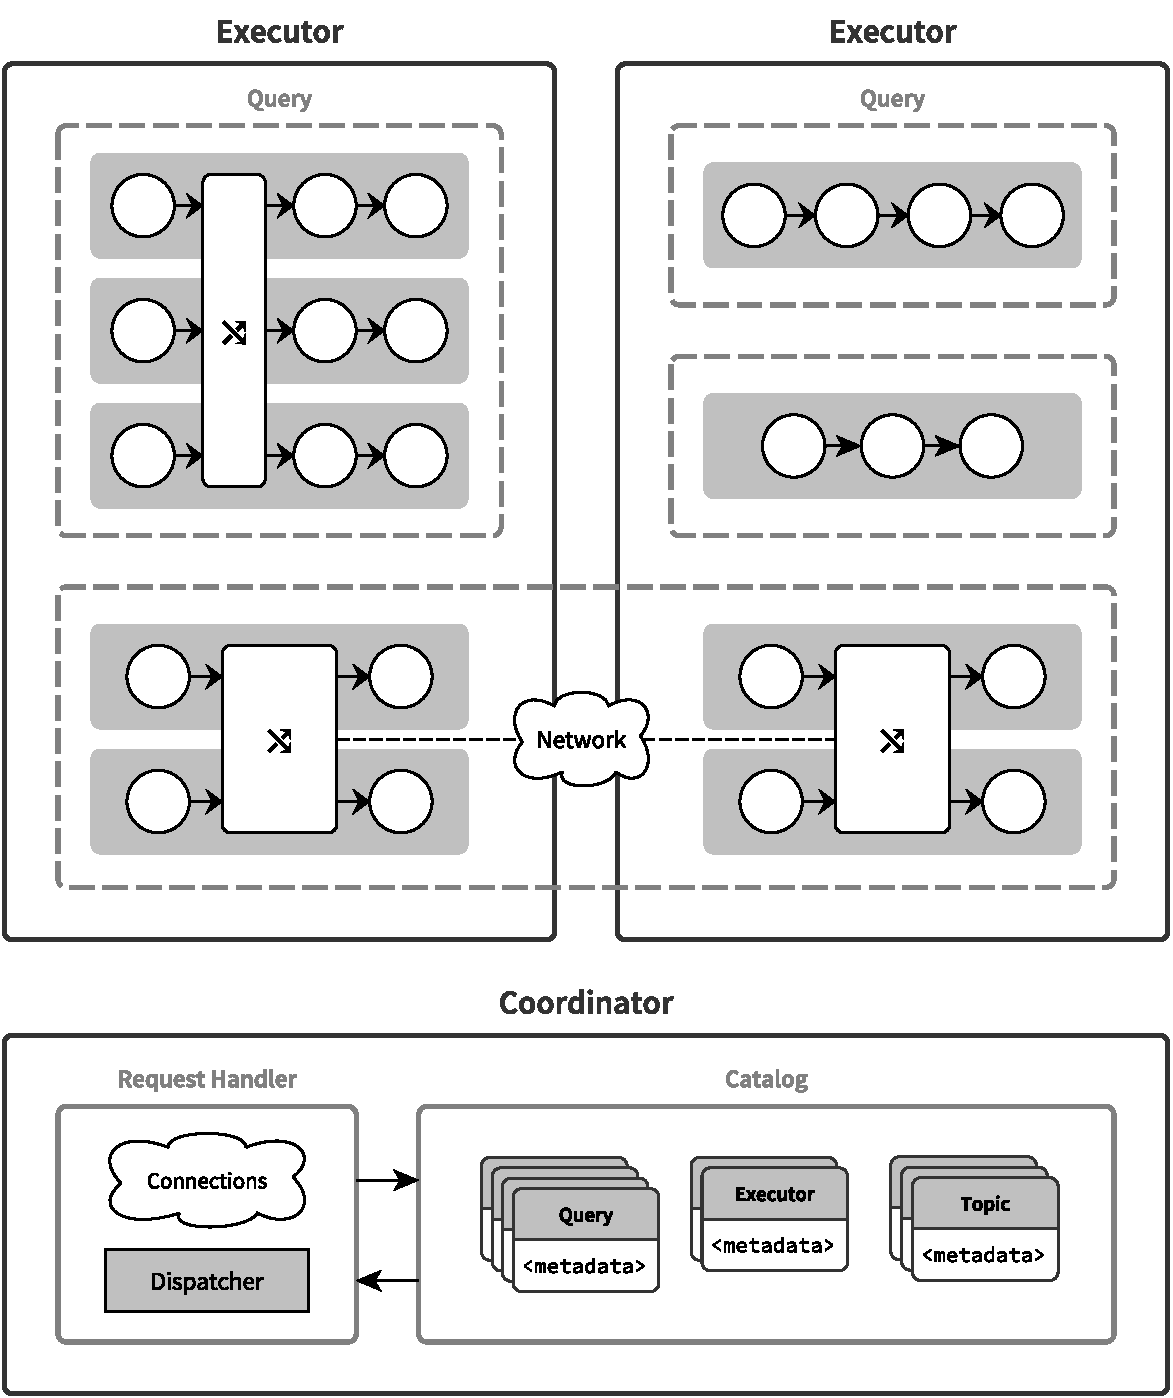
\includegraphics[width=1\textwidth]{figures/components}
  \caption[System architecture.]{ Queries (dashed boxes) consist of one or
  more worker threads (rounded grey boxes) driving the dataflow computation.
  A query might span over multiple executors, make use of the network for message exchanges
  between the workers of a query.\\
  The coordinator maintains a connection to every  executor and every query process.
  The state of the whole system is stored in the catalog.}
  \label{fig:components}
\end{figure}

\clearpage

\section{Queries}

A query is a Timely program managed and executed by our system. Like
standalone Timely Dataflow programs, queries are written in Rust by using the
Timely Dataflow library: The dataflow graph is constructed by connecting
Timely's operators (vertices) to stream objects (edges).

In order for a Timely Dataflow program to become a runnable query on the system,
it needs to link against our query system library. Instead of using Timely's 
initialization functions, a query registers its computational logic with our
\lstinline{timely_query::execute} function.
This function not only performs the initialization of the query according
to submission requests, it also provides additional functionality to interact
with the coordinator. Other than this, there are no restrictions on what the
query program does, it is free to execute arbitrary code.

\begin{lstlisting}[caption={[Example query.]Example query which creates a stream of integers,
filters out all odd numbers and then prints the rest.}]
extern crate timely;
extern crate timely_query;

use timely::dataflow::Scope;
use timely::dataflow::operators::{Filter, Inspect, ToStream};

fn main() {
    timely_query::execute(|root, coordinator| {
        root.scoped::<u32, _, _>(|scope| {
            (0..100).to_stream(scope)
                .filter(|x| x % 2 == 0)
                .inspect(|x| println!("hello {:?}", x));
        });
    }).unwrap();
}
\end{lstlisting}



Timely implements a data-parallel approach for its computation. This is done by
instantiating the dataflow graph on multiple worker threads, where each worker
drives the computation of its local instance, and the data is distributed by
user-provided sharding functions. Workers can be distributed among multiple
machines, where the computation consists of multiple operating system processes
which are communicating with each other over the network. Such an
operating system process might host multiple worker threads.

\begin{figure}[htb]
  \centering
    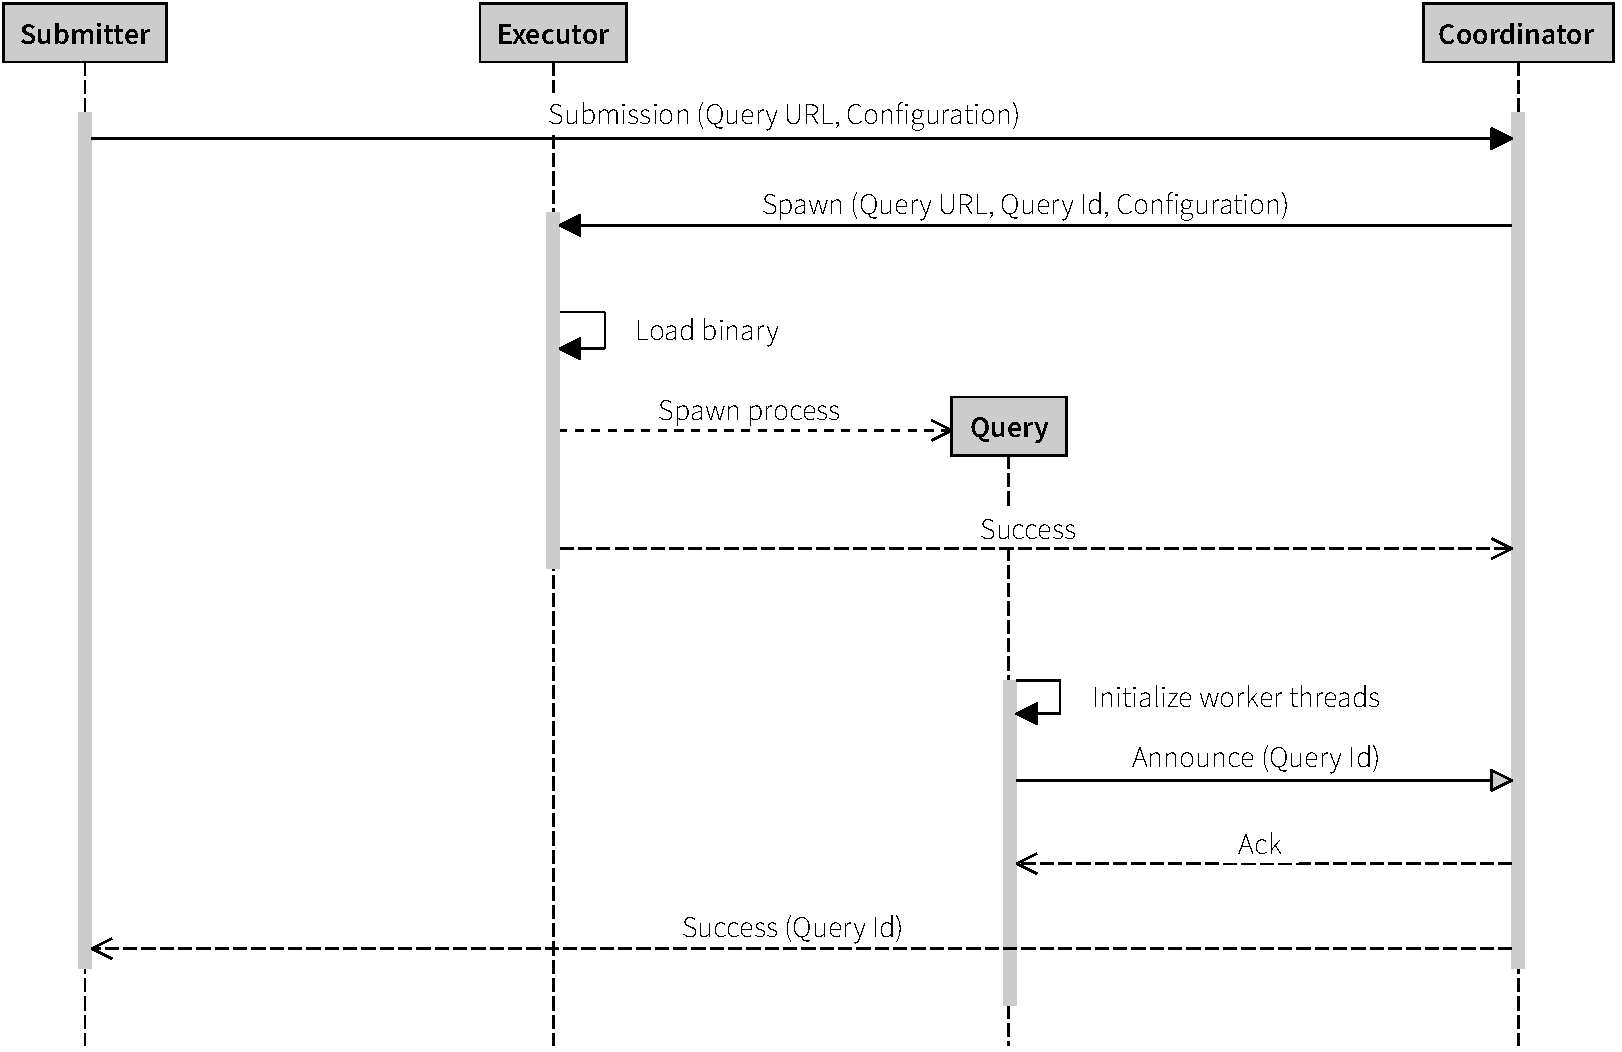
\includegraphics[width=1\textwidth]{figures/spawn_singleprocess}
  \caption[Query submission with single process.]{Submission of a query on a single executor.
  Only once the spawned query announces itself at the coordinator is it considered running.}
  \label{fig:subsingle}
\end{figure}

\section{Executors}

The spawning and direct supervision of query processes is not done by the
coordinator itself, but is offloaded to designated processes called executors.
This choice allows for more flexibility regarding query execution and the
management of available resources. Since executors can be dynamically added
to the system, and with some limitations also be removed again, they provide
a way for adding new machines to the cluster running our system. The catalog
maintains the pool of available executors which are participating in the system.

As a timely program can span over multiple machines, a query might span
over multiple executors. The placement of a query on the available executors
is performed by the coordinator, based on the users request.
We currently implement a naive approach to query placement, where the executors
are chosen randomly if the user does not manually specify a placement. A more
sophisticated scheduling, which for example could include load balancing,
has to be investigated.

Another feature of executors are that they define on how queries and their
worker threads are supposed to be executed. When an executor joins
the system by introducing itself to the coordinator, the executor also informs
the coordinator about the execution format it supports. In the current
implementation, executors only support the execution of queries in the form of
native operating system executables.

When spawning such an executable, the newly spawned query process and the
executor coordinate. The executor supplies the newly created process with the information
it needs in order to participate in the system. This includes the query's own identifier,
the address of the coordinator, the addresses of any peer processes belonging to the 
same query, and the number of worker threads to spawn inside this process.

Executors are also responsible for fetching any query binaries they are supposed
to spawn. When submitting a new query, the submitter has to provide coordinator
with the URL of the binary. This URL is forwarded to participating executors,
which will use it to download the query binary. 

Since executors serve as a provider for computational resources such as machines,
there is typically a one-to-one mapping between executors and the machines they
are running on. This however is not a requirement of the system, the deployment of
executors is left to the user. Similarly, the user is free spawn multiple
processes belonging to the same query on the same executor if they wish to do so.

Since operating system processes can outlive their parent process, executors can
be removed from the system while the queries spawned by the executor are still
running. In this case, the coordinator removes the terminating executor from
the pool, disallowing any future queries to be hosted on the removed executor.

\paragraph{Future Considerations}

The current implementation of executors which run queries in their own separate
process is not the only possible implementation choice.
Alternative implementations could for example host multiple queries
within the same process, by dynamically loading the query's code into an already
running process and run it on a preemptive OS thread. This would allow queries
the interchange of objects without the need for data serialization. Given
the implementation of Timely's operator scheduling, cooperative scheduling
of multiple worker threads within a single operating system thread could also
be implemented for certain queries where its input is managed by the system.
\section{Coordinator}

The purpose of the coordinator is to manage all components of the system. It
provides an interface for users to submit new queries and inspect the current
state of the system. In order to receive commands and report their internal state,
every executor and query process maintains a network connection to the coordinator.

Bookkeeping of the system is done by the coordinator in the catalog. The
catalog is a datastructure which contains all information about the available
executors, the running queries and their workers. 

\subsection{Submission}

A query is submitted to the coordinator as a binary executable. A submission
consists of an URL and format of the query binary, as well as the runtime
configuration for the workers. The runtime configuration specifies the amount
and distribution of the worker threads which will drive the query.

Optionally, a human-readable description of the query,
as well as the command-line arguments to be passed to the executable can be
provided.

When handling a new query submission request, the coordinator will assign a
unique identifier to the incoming query, and then select a
matching number of executors for the query to be spawned on. The selection
of executors is based on the runtime configuration provided by the submission
request.

The coordinator plays an important role when spawning new queries. After
issuing query spawn requests to the executors, it waits for all query processes
to register themselves at the coordinator before they begin their computation.
Only then the query is considered active and the submission request
is reported to be completed.


\section{Sharing Data Streams}

Dataflow programs typically work on streams from external sources. As the same
data source might be of interest for different dataflow computations, it seems
appropriate to also manage input data streams in our system as well. Furthermore,
input streams might not only come from external sources: A dataflow computation
might produce an intermediate or final output stream which could be of interest
for other queries. These assumptions motivate us to extend our system with a
mechanism to allow queries to expose their data streams for consumption by other
queries.

\TODO{Motivation for topic-based pubsub:

- discoverability and type-soundness of topics, type-based reflection hard

- decoupling from producer and consumer (no storing of old data, buffering done by library)

- dynamic adding and removal of topics decoupled from queries lifetime}

We loosely adapted the terminology of publish/subscribe systems: Using the
\emph{publish} operator, a query can expose one of its stream
(an edge in the dataflow graph) to other queries, which in turn then \emph{subscribe}
to it. The list of all published topics is stored at in the catalog.

\subsection{Topics}

A topic has the following properties, which are all stored in the catalog
and can be accessed by other queries.
\begin{description}
\item [Identifier] A unique identifier for the topic instance.
\item [Name] When publishing a stream, the publisher has to assign a name to it.
Queries use this name to refer to topics they want to subscribe to. There might
be only one topic with a certain name at a time, however names can be reused if
topics are unpublished.
\item [Data type] A descriptor of the data type of the stream published in this
topic. Timely's streams are typed channels, therefore so are topics.
\item [Address] An address to which the subscribers connect in order to received
the contents of the published stream.
\end{description}

While every publication and subscription request is disclosed to the coordinator
and the catalog contains a list of all existing topics, the
actual exchange of data happens directly between queries. When a query subscribes
to a topic, it receives the address of the topic's publisher from the coordinator
and directly connects to it.

\subsection{Stream Publisher}

A stream publisher is a Timely operator which exposes a Timely stream as a topic. When
creating it, the query author has to assign a name for the topic under which the
input stream will be published. As with all other Timely operators, the publisher
operator is instantiated on all worker threads. However, the user can choose
whether all worker streams are merged into a single topic before publishing, or
if each worker publishes its own topic. The latter option implicitly exposes
the data sharding strategy of the publishing query, allowing the workers of
the subscribing query to exploit this partition scheme.

\subsubsection{Collection Publisher}

\begin{comment}
This however might be too limiting for some use cases where previously published
data might is essential for a full understanding of the data stream. A simple
solution for this problem would be to buffer the stream at the publisher
and replay it to every incoming subscriber. While simple, this approach
would be wasteful in cases where the data in the buffer becomes stale and
irrelevant to future subscribers. \TODO{this doesn't motivate \emph{unordered}
multisets}
\end{comment}

Normally, publishers are not buffered, meaning subscribers will
not receive any data which was produced before they subscribed to a certain
topic. This is the same as in many other publish/subscribe systems, where
synchronization between publishers and subscribers is decoupled as well. \cite{pubsub}

However, in streams where the contents of the stream describes changes of a certain
state, it is essential for stream consumers to know the state of the source at
the beginning of the stream in order to make sense out of it.

For this reason, we introduce a different kind of publisher which publishes
\emph{collections} instead of streams. A collection is a typed, unordered
multiset maintained by the publisher, possibly representing state it would
like to share with subscribers.

Upon creation, a collection publisher contains an empty collection.
When the publishing query mutates the collection by adding or removing elements,
these changes are propagated to the subscribers. When new subscribers connect
to this publisher, they will initially receive a list of all currently contained
elements. This way, all subscribers eventually maintain the same view of the
data collection.

From the subscribers point of view, a topic published by a collection publisher
is not inherently different from a normal topic: After subscribing, it will
observe a continuous stream of data. The difference is in the data type of the
stream, it will be of tuples of the format $(\texttt{Data}, \delta)$, where
\texttt{Data} is an element that can be stored in the multiset and $\delta$ 
denotes the amount of elements that have been added or removed from the set.
This format
is compatible with the notion of collections in Differential Dataflow, allowing
subscribing queries to further process the collection in a convenient manner.

\subsection{Subscriber}

In order to subscribe to a topic, the subscribing query has to provide the name
of the topic it is interested in. This involves a name lookup which can optionally
be blocking: If a requested topic does not yet exist, the coordinator will add
the subscriber to a wait list. Once a corresponding topic is published under that
name, the coordinator will inform the subscriber about this topic. 

The subscribing query might use different timestamps in its dataflow graph
than the publisher, thus it is the subscribers responsibility to re-add
timestamps to the received stream. 

\subsection{Alternative Approaches}

\subsubsection{Capture \& Replay Operator}

The Timely library also offers the capture and replay operators which serve the
purpose of sharing data between queries. With the capture operator, all timestamp,
data and event records are collected and stored in one dataflow computation,
and can then be replayed in another one.

The implementation of the replay operator requires it to use the same timestamps
as the capture operator, forcing both queries to have a similar structure
in their dataflow graph, as a timestamp received at an operator is defined
by its surrounding scope. Another feature of the capture/replay operator pair
is that they will replay the whole stream from beginning to end, requiring the
capture operator to either buffer its incoming data or wait for the replaying
query to connect to it. 

Both these requirements stem from the fact that the replay operator not only
replays the data stream, but also all progress tracking events, including
notifications. In our system, we opted for a more dynamic approach, where
producing queries are allowed to discard data if there are no consumers, and
where consumers use the streams as inputs for their own computation,
allowing them to assign their own timestamps to the data stream.

It is the user's task to provide a communication channel between capture and 
replay operators. Common channel include Rust's thread-safe FIFO queues or
TCP sockets. In general it can be said the capture/replay operators result
in a more tightly coupled system than publish/subscribe pairs.


\cleardoublepage
\chapter{Implementation}\label{ch:impl}

In this chapter, we discuss the implementation of the individual components
presented in the previous chapter. We also present some shared implementation
features, such as the common request/response protocol used for the
communication between the different components and the coordinator.

\section{Query Library}

As discussed in the previous chapter, queries link against a small wrapper library
which allows submitted Timely programs to participate in our system.
This library performs the initialization of the dataflow computation,
announces its readiness at the coordinator and provides methods for
publishing and subscribing to topics.

For the query to announce itself in the system, the query author must eventually
call the \lstinline{timely_query::execute} function. This function
mirrors Timely's own \lstinline{execute} function in that it performs the execution
of the computation. In contrast to Timely however, our version does not provide
any means to specify the runtime configuration of the execution. This information
is specified by the user at submission time and directly provided to the query library
by its hosting executor. The current implementation of the executor passes
this information down to the query library in environment variables. 

Using this information, the query process connects to the coordinator and registers
itself by providing its identifier and the group of workers it will host. Once
all worker groups have successfully registered themselves at the coordinator,
the coordinator replies with a randomized token which is used to associate
the registered processes with the query.

The initialization of the Timely worker threads and the allocation of the
communication channels among them is by the library done using
\lstinline{time\-ly_\-com\-mu\-ni\-ca\-tion} the same way as it would be done
in a standalone Timely program. For this reason, our query library needs to
translate the information provided by the executor into Timely's own format.

Our query library provides an interface for worker threads to
publish or subscribe to topics. For this reason, every worker thread gets
a handle for the connection to the coordinator. Access to the
publish \& subscribe system is provided through a set of remote
procedure call stubs which are described separately in section~\ref{sec:pubsubimpl}.

\section{Executor}

The current implementation of the executor is relatively simple, it is a
process that spawns child processes on behalf of the coordinator, enabling
the execution of new queries on remote machines.

In order to add a new machine to the cluster, the user has to deploy the executor
binary on the new host, specify the address of the coordinator and then launch
the executor binary. The executor will register itself at the coordinator, which
in turn assigns a unique identifier to the connecting executor. Once connected to the
coordinator, the executor listens for incoming spawn requests. If such a
request arrives, it fetches the binary from the specified source and launches
it as an operating system process. During submission, the user can specifying
command line arguments which are provided to the query binary here as well.

The executor has to inform the spawned binary about its assigned query identifier,
the address of the coordinator and the address of any peer processes. In the
current implementation this is simply done by the executor writing this information
into the environment variables of the spawned query.

The executor currently uses the process spawning functions provided in Rust's standard
library, which at present offer all features we need, and are available on
all supported operating systems. As we will discuss in later chapters,
more sophisticated, platform-specific process control and supervision mechanisms
could be added in the future.

When submitting a new query, the submission must contain an URL to the binary.
The URL scheme determines how the binary is fetched by the executor. In the
current implementation, this can either be a filesystem path directly accessible by the
executor process (e.g. over a shared network folder), or the binary can be provided
over a raw TCP stream. More advanced download schemes can be easily added in
the future.

% TODO talk about the removal of queries
% TODO talk about stdout forwarding

\section{Coordinator}

As the central component of our system, the coordinator performs a rich
set of tasks. These involve handling submission requests to spawn new queries,
but also handling publication and subscription requests from existing queries.
It is the central authority on the current system state, i.e. it maintains
a list of all running queries and executors, but it also tracks all existing
publications and subscriptions. It exposes this information through the catalog.

Because most components interact with the coordinator, its internal implementation
is not without challenges, particularly when dealing with multiple concurrent events.

Before we discuss the details of its implementation, we provide a
brief overview of the internal architecture of the coordinator: To other
components, the coordinator exposes a request/response-based interface on a
predefined networking port. It listens for incoming connections on that port
and then waits for the connected clients to send their requests. Once a request
is received and decoded, it is forwarded to a central request handler.
This request handler contains the central logic of the coordinator, keeps
track of unfulfilled requests, and informs the catalog to announce changes
in the system state.

\subsection{Dealing with Asynchronous Tasks}
Our initial prototype of the coordinator used a multi-threaded approach for dealing
with multiple clients at the same time, and used message passing between threads
to avoid directly exposing shared state. However, many requests handled by
the coordinator require it to wait for external events, and thus a form of
cooperative task management is needed.

We initially used a continuation-passing style for splitting blocking requests into
non-blocking subtasks. However, due to Rust's memory ownership model, we found that
this approach often resulted in manual \emph{stack ripping} \cite{stackmgmt},
which made code both hard to read and inconvenient to write.

This motivated us to re-design the coordinator around a central task dispatch loop, which
allows us to multiplex many asynchronous tasks within the same thread. We decided to adapt
an external library called \lstinline{future-rs} \cite{futuresrs} for this purpose.
It provides an expressive interface for dealing with asynchronous tasks based
on the concept of \emph{futures}. Futures (sometimes called promises, eventuals
or deferred objects) are proxy objects for absent values, which eventually will
be provided through some asynchronous event.
The \lstinline{future-rs} library provides combinators for chaining futures
together or waiting on multiple futures at the same time. Actions on completed
futures are expressed as closures. This approach does not completely eliminate
stack ripping, however the fact that the completion handlers are chained together
allows for much more maintainable and sequentially looking code. Listing~\ref{lst:fnsubscribe}
shows how futures can be used when executing potentially blocking requests.

A unique aspect of the implementation of \lstinline{future-rs} is that its futures
need be polled in order to make progress, instead of proactively being called
by event sources. When a future is polled, it checks if any pending events
have occurred. If so, it dispatches any pending completion handlers. 
It is the users responsibility to ensure that futures are being
polled. This is typically done by registering the future in an event loop,
which will repeatedly wait for events to occur before polling its registered
futures.

\subsubsection{Task Dispatcher}
The \lstinline{future-rs} library itself provides a set of primitives to
create and combine futures. It also provides abstractions for expressing which
events a future is waiting for, and expressing the occurrence of events. It
does however not provide an actual implementation of an event loop. Our implementation
of the coordinator thus provides a simple task dispatcher whose sole purpose it is
to wait for events to occur and poll registered futures accordingly.

To avoid having to pass around a handle to the dispatcher, we store its 
list of pending futures in thread local storage. The public interface consists 
of two free-standing functions, \lstinline{async::spawn} for registering
futures which are to be completed, and \lstinline{async::finish} which initializes
the dispatcher loop and then waits for its termination.
\lstinline{async::finish} accepts an initial future which acts as the root task.
The motivation for the names in this interface comes from the fact that model
each concurrently running task as a chain of futures, basically treating them as
coroutines.

Listing~\ref{lst:coorddispatch} shows an example of this. Our networking layer
models the server socket as a future which yields a stream of incoming connections.
Each connection itself is then maintains a queue for incoming requests, which is
also modeled as a future, allowing the user to specify actions to be taken
once a request is received.

\begin{figure}[htb]
\begin{lstlisting}[caption={[Connection handling at the coordinator]%
Accepting and dispatching incoming connections. The actions specified
in \lstinline{for_each} and \lstinline{map_err} are invoked by the
task dispatcher when the corresponding events (such as new incoming connections,
new incoming requests or errors during request handling) occur.},label={lst:coorddispatch}]
// a future yielding a stream of accepted connections
let listener = network.listen(9189);
// define the action to be executed for each incoming connection
let server = listener.for_each(|connection| {
    ...   
    // this action is invoked for each incoming request
    let client = requests.for_each(move |request| {
        // decode and dispatch request 
        match request.name() {
          "Subscribe" => {
            let (req, resp) = req.decode::<Subscribe>();
            // forward the request to the request handler,
            // which will return a future (see Listing 4.2)
            let subscribe = request_handler
              .subscribe(req)
              .then(|result| Ok(resp.respond(result)));
            // complete this task asynchronously
            async::spawn(subscribe);
          }
          ...
        }
        ...
    }).map_err(|err| {
        // futures can also yield error values
        // which are handeled separately
        error!("failed to dispatch request: {:?}", err)
    });

    // handle client asynchronously
    Ok(async::spawn(client));
});

// drive the event loop to completion
async::finish(server);
\end{lstlisting}
\end{figure}

\begin{figure}[p]
\begin{lstlisting}[caption={[Handler for blocking subscription requests]
Example how a future is created for the subscription request. Depending
on whether it can be served immediately or not, different kinds of futures
are returned. Bookkeeping for still pending requests is done with completion
handles. Upon publication of a requested topic, any pending subscriptions will
be completed by calling \lstinline{lookup.complete()}.},label={lst:fnsubscribe}]
struct RequestHandler {
  catalog: Catalog,
  // list of pending lookups
  lookups: HashMap<String, Vec<Complete<Topic, SubscribeError>>>,
  ...
}

impl RequestHandler {
  pub fn subscribe(&mut self, request: Subscribe)
    -> Box<Future<Item=Topic, Error=SubscribeError>>
  {
    // extract arguments from the request
    let query = request.query.id;
    let name = request.name;
    // first, check if the topic actually exists
    if let Some(topic) = self.catalog.lookup(&name) {
      // if so, insert a new subscription into the catalog
      self.catalog.subscribe(query, topic.id);
      return futures::done(topic).boxed();
    } else if request.blocking {
      // allocate an unresolved future and a completion handle
      let (lookup, result) = promise();

      // to be executed once the topic exists
      let handler = self.handle();
      let result = result.and_then(move |topic| {
        handler.catalog.subscribe(query, topic.id);
        Ok(topic)
      });

      // register the completion handle for pending lookups
      self.lookups.entry(name).or_insert(vec![]).push(lookup);

      return Box::new(result);
    } else {
      // non-blocking subscription request, fail immediately
      let err = SubscribeError::TopicNotFound;
      return futures::failed(err).boxed();
    }
  }
\end{lstlisting}
\end{figure}

\subsection{Maintaining Shared Mutable State}

The nature of the coordinator requires it to mutate its internal state on
behalf of the connected clients. This means that we have to provide each
connection handler with mutable access to the central request handler. 
In addition, we also want to keep track of the requests submitted by
each connection, so we can clean up any associated global state if a connection
disappears.

For this reason, we provide a wrapper type for accessing the methods of the
request handler. For each connection, this proxy maintains a simple list of
identifiers for objects that are conceptually owned by the connection, ensuring that the state is
removed from the catalog once the connection drops. Examples of this are the removal
of disconnected executors from the catalog, or the depublication of topics
owned by crashed queries. The proxy object internally uses Rust's
\lstinline{RefCell<T>} type to dynamically ensure the strict language
rules on shared mutability.

\clearpage

\subsection{Catalog}

The purpose of the catalog is to maintain and expose the current state of the
system. It tracks the addition and removal of executors, queries, topics,
publication and subscriptions and exposes them in collection topics according
to the schema shown in Figure~\ref{fig:model}.

\begin{figure}[htb]
  \centering
    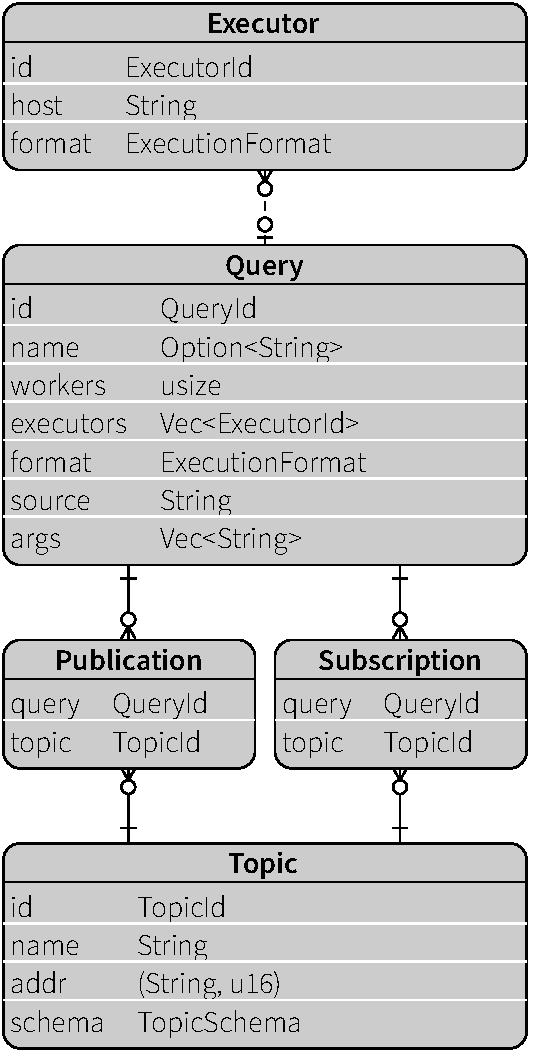
\includegraphics[width=0.5\textwidth]{figures/model}
  \caption[Schema of the catalog]{Schema of the catalog. All five data types
  are published as a collection topic, allowing users to follow state changes
  in the system.}
  \label{fig:model}
\end{figure}

The catalog itself only exposes this data. It is mutated and queried by the
request handler in order to fulfill the submitted requests.


\clearpage
\subsection{Publishers \& Subscribers} \label{sec:pubsubimpl}

The query library exposes the publish and subscribe functionality. The following
API is used for publishing and subscribing to Timely streams.

\begin{figure}[htb]
\begin{lstlisting}[caption={[Publish \& subscribe interface]
The interface for publishing and subscribing Timely streams.
The \lstinline{NonStatic} bounds on the data and timestamp
parameters are required for safe serialization described in \ref{sec:serialization}.
}]
pub struct Coordinator {
  /* hidden handle to request queue */
}

impl Coordinator {
  pub fn publish<S, D>(&self, name: &str, stream: &Stream<S, D>,
    part: Partition) -> Result<Stream<S, D>, PublicationError>
      where D: Data + NonStatic, 
            S: Scope,
            S::Timestamp: NonStatic;

  pub fn subscribe<T, D>(&self, name: &str, cap: Capability<T>) 
    -> Result<TimelySubscription<T, D>, SubscriptionError>
      where T: Timestamp + NonStatic, 
            D: Data + NonStatic;
}
\end{lstlisting}
\end{figure}

\subsubsection{Publisher}

The \lstinline{publish} function takes a direct reference to a Timely
\lstinline{Stream<S, D>}. These stream handles, which are only available during
the dataflow graph construction phase, allow us to instantiate our own publish
operator on the stream.  The instantiated publish operator will push its
incoming data as well as its current frontier to any subscribers. 

Once the operator is inserted into the dataflow graph, the \lstinline{publish}
stub issues a registration request to the coordinator, which will result in the
creation of a topic for other queries to subscribe to.

The partitioning argument on the API specifies whether all streams
shall be merged into a single topic, of if every worker publishes its own stream.
Merging of the stream is done using Timely's partitioning functions. 
In the second case, the identifier of the publishing worker is appended to the
name of the topic. 

\vspace{5em}

\begin{figure}[h!]
\begin{lstlisting}[caption={
Publishing partitioned topics.
}]
timely_query::execute(|root, coord| {
    root.scoped::<u64, _, _>(|scope| {
        let i = scope.index();
        let numbers = (i*100..(i+1)*100).to_stream(scope);

        // results in `n` topics:
        //    "numbers.0", "numbers.1", .., "numbers.n"
        coord.publish("numbers", &numbers, Partition::PerWorker)
             .expect("failed to publish topic");

        // filtering performed by each worker in parallel
        let primes = numbers.filter(|x| x.is_prime());

        // results in a single merged topic called "primes",
        // published by worker with index 0
        coord.publish("primes", &primes, Partition::Merge)
             .expect("failed to publish topic");
    });
})
\end{lstlisting}
\end{figure}

\paragraph{Collection Publisher}

In addition to the stream publisher, we also provide the so called collection
publisher. It has a similar interface for publishing, but it requires the
type of the incoming stream to deliver \lstinline{(D, i32)} tuples, where
the integer denotes the amount of elements that have been added or removed from
the collection.

\begin{lstlisting}[caption={[Collection publisher interface]
}]
impl Coordinator {
  pub fn publish_collection<S, D>(&self, name: &str,
    stream: &Stream<S, (D, i32)>, partition: Partition)
    -> Result<Stream<S, (D, i32)>, PublicationError>
      where D: Data + NonStatic, 
            S: Scope,
            S::Timestamp: NonStatic;
}
\end{lstlisting}

Internally, the publisher maintains a copy of this collection. This is required
for new subscribers, which must be informed about the contents of the collection
when they connect.

\paragraph{Implementation Details}

Both publishers share the same underlying logic which accepts incoming connections
from subscribers and provides notifications for disconnected clients.

Internally, this logic also make use of the \lstinline{future-rs} library, 
since futures have also been integrated in our networking layer.
Inside the coordinator the polling is done by the task dispatcher. For the futures
inside our publish and subscribe operators however we make use of the fact
that Timely itself also uses polling-based scheduling. Every time the publish operator
is scheduled by Timely, it can poll the networking layer to be informed
about newly accepted or disconnected subscribers.

Note that even though each subscription request is disclosed to the coordinator
by subscribing queries, publishers are not informed by the coordinator about new subscribers. Publishers
see new subscribers only once they connect to the publisher's network socket. 
The information stored in the catalog is only exposed for inspection by the user.
Figure~\ref{fig:pubsubseq} shows hows the sequence for publishing a new topic.

\begin{figure}[htb]
  \centering
    \vspace{1em}
    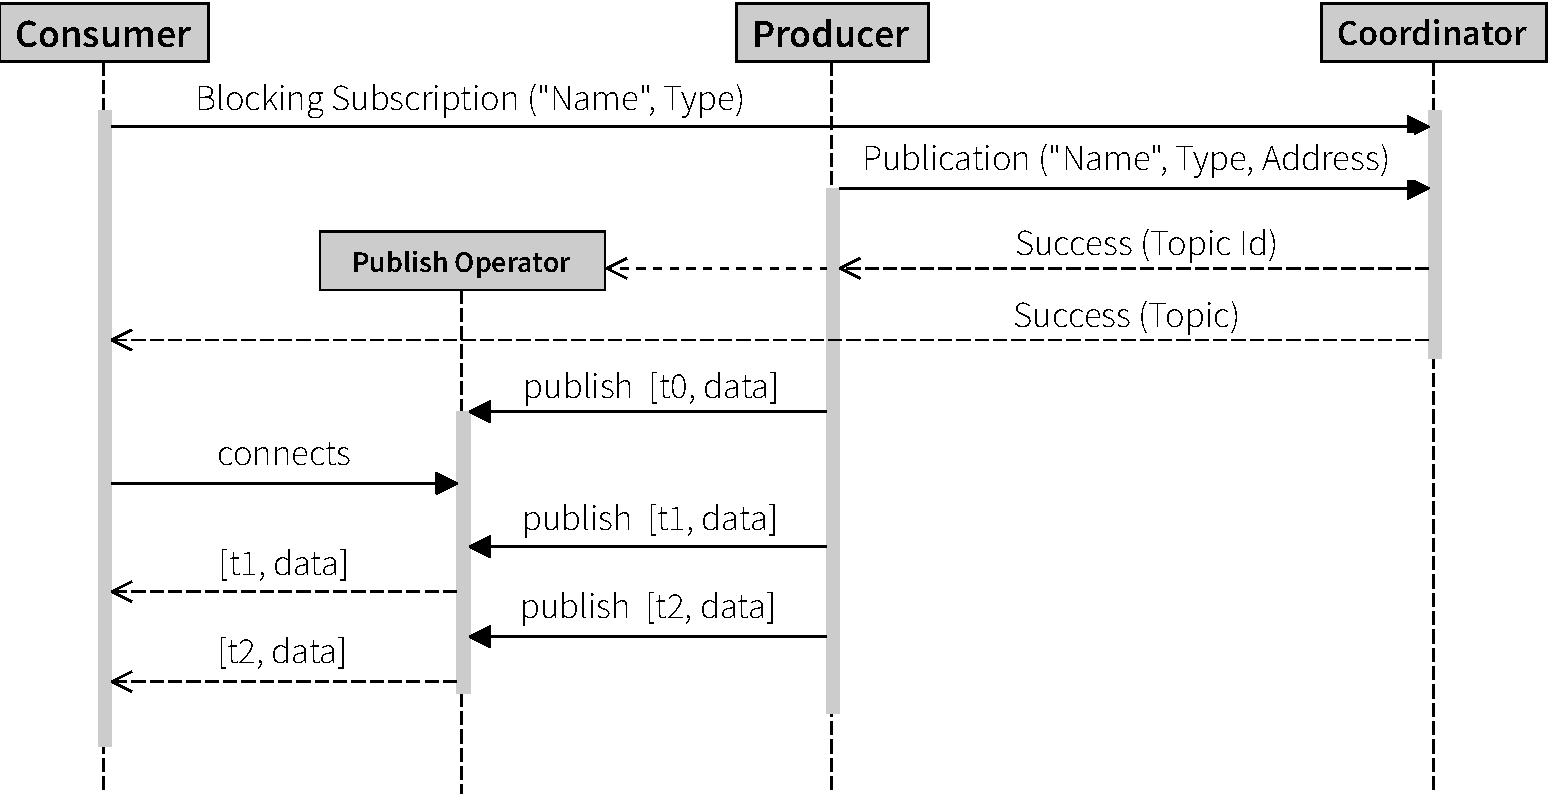
\includegraphics[width=1\textwidth]{figures/pubsubseq}
  \caption[Publish/subscribe sequence diagram]{Sequence diagram for the publish/subscribe procedure. Any data
  produced before the subscriber connects might be lost.}
  \label{fig:pubsubseq}
\end{figure}

\subsubsection{Subscriber}

In contrast to the publisher, the current implementation of the \lstinline{sub\-scribe}
function does not directly instantiate a Timely operator, but returns a subscription
handle which is used to read data from the topic.

There are two reasons for this choice: First, Timely requires that an operator
is instantiated on every worker, such that all instances of the dataflow graph
are identical. However, the amount of topics a query would like to subscribe
to, and the amount of workers it allocates might not match. Thus, the API
quickly becomes complicated, as we would need to provide a way for the 
query author to map topics to operator instances.

Second, Timely's operator contract requires that an operator instance announces
the internal initial capabilities it holds, and, more importantly, the initial
capabilities of its peers. To support this would require some synchronization
between the subscribers, as they have to exchange the initial frontier they
observe at their topic.

Instead, we decided to base our subscription progress tracking on Timely's new
capability handles. The recently added \emph{unordered input operator} allows
a query to feed a computation from data with unordered timestamps. This operator
exposes a root capability for the earliest possible timestamp, allowing the user
to derive capabilities for newer timestamps from old ones. The frontier
is advanced by dropping the capabilities for timestamps for which no more data
is pending.

Based on the progress tracking information delivered by the publisher, the
subscription handle will automatically derive new capabilities for incoming
data and drop old ones if the frontier advances. The user however has to
provide the initial root capability for the input.

\begin{figure}[htb]
\begin{lstlisting}[caption={[Typical use of the subscription handle]
Typical use of the subscription handle. This query subscribes to a single topic of
strings, with \lstinline{u64} being the type of the timestamps.
},label={lst:subhandle}]
timely_query::execute(|root, coord| {

    let (mut input, cap) = root.scoped::<u64, _, _>(|scope| {
        let ((input, cap), stream) = scope.new_unordered_input();
        // stream.operators(..)
        (input, cap)
    });

    let topic = coord.subscribe::<_, String>("example", cap)
                     .expect("failed to subscribe");

    for (time, data) in topic {
        let session = input.session(time);
        session.give_content(&mut Content::Typed(data));
        root.step();
    }
})
\end{lstlisting}
\end{figure}

In queries which use multiple workers, the query author can programmatically
encode which workers subscribe to which topics, as the code outside the
graph generation is allowed to conditionally decide if and how it wants to call
the subscribe function. This functionality is required as there is not
always a one-to-one mapping between published topics and workers at the
subscribing query, and expressing the assignment in arbitrary Rust code
gives the most flexibility to the query author.

Because the root capability can be cloned, this interface also allows the user to
interleave the data from a topic with other data, for example by merging
multiple topics at the input. Our subscription handle implements the
\lstinline{futures-rs} stream interface, allowing the client code to wait for
data from multiple subscriptions at once.

\clearpage
\section{Shared Communications Layer}

For the remainder of this chapter we discuss the networking layer of our system,
which is used by all components to implement their services.

\subsection{Messaging}

Our system consists of potentially many distributed processes. These processes
are running concurrently, are dynamically added and removed from the system
and are communicating with each other. In order to deal with the inherent
complexity of such a system, we adopted an actor-model like approach for our
networking implementation.

Actors in our system include processes like the coordinator, the executors 
and the query processes. But we also treat the publish or subscribe operators
as actors, as they directly interacting with our system.

To support this kind of model, our networking layer also works in terms of
asynchronous messages. In contrast to Timely's own networking layer which also
provides a similar abstraction, we cannot assume a fixed number of components.
In order to establish a connection between two components, one of them has to
take on the role of the server, while the other one acts as a client. Two
queues are allocated per connection on each side: one for incoming messages
and one for outgoing messages. This enables messages to be sent asynchronously
in both directions. Network failures are signaled in the queue for incoming
messages. Currently, Rust's standard library TCP sockets are used as the
underlying transport mechanism, however the system could easily be extended to
support alternative transport layers as well.

\subsection{Request \& Response Messages} \label{sec:reqresp}

While the abstraction of single messages is sufficient for implementing the
mostly unidirectional messaging paradigm of the publish-subscribe implementation,
most other communication in the system follows a request-response pattern,
e.g. any communication with the coordinator.

For this reason, we implemented a request-response multiplexer on
top of the plain message channels. This multiplexer allows both sides to have
multiple requests in flight while waiting for the corresponding responses,
which can be delivered out of order.

In order to differentiate between different kind of requests and also ensure a
well-typed response format, request payloads have to implement the \lstinline{Request}
trait. The associated name is used for decoding, while the associated \lstinline{Success}
and \lstinline{Error} types specify what kind of payloads are valid for the response.
This allows the response for a given request \lstinline{R} to be represented by
Rust's \lstinline{Result<R::Success, R::Error>} type.

\begin{lstlisting}[caption={[Request trait]In order for a type to be used as a
request message, it needs to implement the \lstinline{Request} trait. The name allows
request handlers to differentiate between different types of requests, while the associated
types forces them to issue well-formed responses.
The trait bounds are explained in section \ref{sec:serialization}.}]
pub trait Request: Abomonation + Any + Clone + NonStatic {
    type Success: Abomonation + Any + Clone + NonStatic;
    type Error: Abomonation + Any + Clone + NonStatic;

    fn name() -> &'static str;
}
\end{lstlisting}

\subsection{Serialization} \label{sec:serialization}

For both, the request/response messages as well as messages used in the publish/subscribe
subsystem, we need to serialize the payloads in order to send them over the network.

\subsubsection{Message Buffers}

Incoming and outgoing network data is stored in reference counted message buffers.
This buffer supports multi-part messages, meaning a message contains more than
one serialized object. This is needed for the request/response multiplexer, which
needs to partially decode a message in order to determine to which request it
belongs to. It is also used in the publisher and subscribers, which allows them
to encode and decode the timestamp and the data separately.

Reference counting is an optimization used by publishers, which allows them to
serialize the data only once and share the buffer with all subscribers. Every
outgoing queue to the subscriber only contains a reference to the buffer. Once
the message is written to the subscriber's socket, the reference count is
decreased and the message is deallocated once all subscribers have consumed it.

\subsubsection{Safe Serialization with Abomonation}

Timely itself provides a uses a high-performance serialization library called
Abomonation, implying that all data types sent to a publish operator will be
serializable this way. This makes Abomonation a natural choice as the serialization
format for the messages sent from publishers to subscribers. 

However, Abomonation is neither memory- nor type-safe. There are no safeguards
against deserializing data into an incompatible type, which will result in undefined
behavior. In Timely, such errors are typically avoided since all worker
execute the exact same program code and the streams between workers are
statically typed. In our system however, a publisher might accidentally use
a different version of a library type than the subscriber. Because of this,
we use our own lightweight wrapper around Abomonation. In addition to the raw
serialized bytes, we annotate the buffer with the \lstinline{TypeId} of the
data type. Rust's \lstinline{TypeId} provides an opaque, globally unique
identifier for a given Rust type and its representation. Thus, we can check
if the expected and provided type identifier match before trying to deserialize
a message.

In order for a type to be serialized by our library, it needs to fulfill the
following type bounds: \lstinline{Abomonation + Any + Clone + NonStatic}.

The \lstinline{Any} trait is required to retrieve the type's identifier. The
\lstinline{Clone} trait is used to put deserialized types into the incoming
messages queue and \lstinline{NonStatic} is an auto-trait used to disallow the
creation of eternally valid pointers into temporary buffers. We also take type
alignment rules into consideration when serializing into unaligned buffers. 

\paragraph{Alternative Serialization Formats}

We currently use our safe Abomonation wrapper not only for data in
publish/subscribe system, but also for serializing and deserializing requests
and response messages. This implies that currently all participating components
have to be compiled for the same processor architecture and operating system.

Because of this, our message buffer interface has been designed to use alternative
serialization formats in the future. Besides supporting heterogeneous clusters,
alternative formats might also be useful in the publish/subscribe system:
Schema-based serialization formats would allow subscribers to decode published
data even without static knowledge of its data type.

\cleardoublepage
\chapter{Evaluation}\label{ch:evaluation}



\cleardoublepage
\chapter{Related Work} \label{ch:related}

\section{Related Work}

\subsection{Dataflow streaming engines}

In contrast to the standalone Timely Dataflow library, many state-of-the-art
dataflow streaming engines have been designed and engineered from the start
to run multiple current dataflow computations in a cluster. One of the
goals of this thesis was to provide such functionality for Timely Dataflow
based programs. Thus, in this section, we will mainly focus on the execution
and management aspect running multiple dataflow computations. Less focus is
put on the differences in the programming and synchronization model these 
other systems provide. Our system currently also does not provide any fault
tolerance guarantees. This is also a notable difference our system has compared
to related work, which often put heavy emphasis on providing strong fault
tolerance.

\subsubsection{Spark Streaming}

Spark Streaming \cite{sparkstreaming} is a streaming engine based on the Spark
cluster computation framework. Spark Streaming executes streaming dataflow
computations by turning them into stateless, fault-tolerant batch computations.
These batches are submitted as tasks to the underlying Spark engine. \cite{spark} 

\paragraph{Process Model}

In Spark, computational tasks work is modeled as transformations on partitioned
collections of records called \emph{resilient distribute datasets}. The
runtime schedules the execution of the transformations on a distributed set of
worker nodes. By tracking the lineage of transformations, Spark is able to
recover computations by reissuing lost transformations. Based on the model,
Spark Streaming models stateful, conceptually continuous dataflow computations
as small stateless microbatches.

This model of execution is very different from Timely's continuous operator
model. In Timely, both the operator scheduling and the data of the
computation are managed directly by the workers themselves, which are hosted
by long living operating system processes. In Spark however, the data and code
is managed by the system. Because of this, Spark is not only able provide strong
fault tolerance by reissuing failed computations, Spark is also able to load
balance concurrently running streams and mitigate stranglers. While we currently
do not offer these features, Timely does achieve much lower latencies than
Spark Streaming, which is mostly enabled by the fact that every Timely
worker manages itself independently.

%TODO driver processs

\subsubsection{Storm \& Heron}

Heron \cite{heron} is the API-compatible successor of the Storm \cite{storm}
streaming dataflow engine.
Both Storm and Heron call their dataflow computations \emph{topologies}, which 
are directed acyclic graphs of spouts (stream sources) and bolts
(stream transformers). Parallelism is achieved by the user specifying the
number of instances for each bolt and spout, as well as the partitioning
strategy between them.

\paragraph{Process Model}

The process model of Storm is very similar to our approach: A topology
(roughly corresponding to a query in our system) is executed by multiple
\emph{worker processes}. These are operating system processes which distributed
over different machines, thus similar to our query proceses. Every machine hosts
a \emph{supervisor}, which not only monitors the local worker processes, but also spawns new worker
processes on behalf of the \emph{Nimbus}, making Storm's supervisors similar to our executors.
The Nimbus is a central process to which new topologies are submitted, mirroring our coordinator.

Heron mostly differs from Storm in its internal architecture. Most notably, in
Heron every spout or bolt now runs in its own operating system process. All processes
belonging to the same topology are grouped together in operating system containers.
The motivation for this change are reported to be better debug-ability
and simpler resource management. The authors also state that their topologies
seldom have more than three stages (i.e. bolts/spouts). We believe that such
an architecture would not make much sense for Timely, as its operators are typically
more numerous and more lightweight.

Another major change from Storm's architecture
is the fact Heron does not have a central coordinating process anymore. Being
a single point of failure and a bottleneck, the Nimbus was considered to be a
flawed design. Heron thus replaces the old responsibilities of the Nimbus by
offloading them into a small set of independent processes. This might be something
to consider for futures extensions to our coordinator.

\subsubsection{Flink}

Flink \cite{flink} is a dataflow streaming engine for directed acyclic
dataflow graphs, however it does have support for iterative dataflows on the
outermost level. Flink interleaves control events with data records, which
are used for progress tracking and fault tolerance, which is done through
snapshots. Progress tracking is implemented with global \emph{low watermarks}, which
denote the minimum timestamp which can be emitted at the sources of the
topology, enabling Flink to perform out-of-order processing.

\paragraph{Process Model}

The runtime architecture of Flink also uses a central process called the
\emph{Job Manager}, which accepts and manages computations submitted by
the client. The Job Manager takes the user submitted code, translates it into
an execution plan and potentially optimizes it.

The computations themselves are executed inside worker processes called
\emph{Task Managers}. Task managers provide a similar function like our executors, in that
they are processes distributed over potentially multiple machines and provide access to
computational resources. They can be dynamically added and announce them selves at the
job manager. However, in contrast to our executors, task managers directly execute the
operators and implements the exchange data between them. In our system, this task is done by the
query library and the Timely runtime. For resource management purposes, each task manager provides
a predefined number of task slots. These typically correspond with the number of CPU cores,
though a single slot might host multiple threads. The available memory is also distributed
equally between the task slots of an task manager. The submitted dataflow computation is split up
in multiple subtasks (typically corresponding to an operator), and each subtask is assigned
to a task slot. Subtasksfrom the same job (i.e. submission) can share a task slot
if the operator supports it, which is useful for example for pipelined operators which don't
require any exchange of data with operators running in other task slots.
Because task managers can have multiple task slots, they can run operators from different
computations within the same operating system process, similar to Spark Streaming. Unlike
Spark Streaming, but like Heron and our system, these operators are however long-lived
and do not migrate to other task slots, as Flink also implements a continuous operator model.

\subsection{Dataflow composition}

\subsubsection{Kafka}

Kafka \cite{kafka} is a distributed platform for accumulating and sharing streams. It provides
a publish/subscribe service for potentially partitioned topics. Producers append
their data to one or more partition, allowing subscribers to read from it.
The data within a partition is stored persistently, allowing subscribers to
read all previously published data sequentially and continue where they left
of in case of failure. The data within a partition is ordered, however there
is no defined ordering across multiple partitions of the same topic. Recent
versions of Kafka also supports the assignment of event timestamps to messages.

\paragraph{Integration with Dataflow Engines}

Both Spark Streaming and Flink provide official connectors for Kafka, allowing
dataflow computations to stream data from or to Kafka topics. Flink supports
the extraction of timestamps from topics, allowing a partition
to contain out-of-order data. Similar to our system, Flink also provides a
mechanism to exact watermarks from Kafka sources, which like our system
is able to unify the progress tracking information from multiple sources.

In some ways, Kafka is very similar to our publish/subscribe as we also expose
potentially partitioned streams from which consumers, such as dataflow programs,
can subscribe to. In contrast to Kafka, we have a strict one-to-one mapping between stream
partitions and topics. Stream partitions in our system are only grouped together
by following naming conventions on the topic name. 
 
Another difference between Kafka and our system is that Kafka's subscribers are
\emph{pulling} data from their source, whereas in our system data is \emph{pushed}
from the source to the subscribers. The implication of this in our
system is that the publisher does not know anything about the progress of the
subscriber, which can lead to back-pressure issues if the subscribers are
slow.

\paragraph{Kafka Streams}
In additions to the above mentioned adapters, Kafka also provides its own
streaming engine called Kafka Streams. It provides a simple acyclic dataflow
model which uses Kafka topics and sources and sinks, thus acting as transformers.
Parallelism is achieved by instantiating the dataflow graph on multiple threads.
Partitioning of the data happens before it is fed to the individual instances
of the dataflow graph.

Like standalone Timely Dataflow, Kafka Streams is implemented as a library. It
is left to the user to deploy and launch instances of the streaming computation.

\subsubsection{MillWheel}

MillWheel \cite{millwheel} is a stream processing framework used to implement
the dataflow model proposed by Google \cite{google}. MillWheel conceptually
treats the whole system as a single dynamic dataflow graph: The nodes of the
dataflow graph are user submitted computations (i.e. operators) that are
invoked by the system on receipt of incoming data. Edges are created by the
user specifying which streams a computation consumes and produces. Streams
have uniquely assigned names.

This makes MillWheel essentially a publish/subscribe system, every individual
operator acts as a subscriber and a publisher. This is slightly different from
our system and other combinations of dataflow systems that use an external
publish/subscribe mechanism: Streams between operators are anonymous until
explicitly published, while in MillWheel all streams used to connect operators
are automatically available by for subscription by third parties.

Another difference to our approach is the fact that MillWheel lets subscriber
specify how a stream should be partitioned before it is delivered to the consumer.
Aggregation and partitioning is done according to keys, i.e. records with the
same key are always delivered to the same computation instance. Different
computations can however use different keys on the same streams, as every computation
needs to provide a key extraction function for each of its input streams.

Computations run on one or more processes distributed over a dynamic set of
machines. The assignment of computations to machines and keys to computations
is managed by the system it self. Because the system manages persistent state
on behalf of the computations, computations for a certain key can be moved
for load-balancing or restarted in the case of failures.

\begin{comment}
\begin{table}
    \myfloatalign
  \begin{tabularx}{\textwidth}{llllll} \toprule
    \tableheadline{Feature} & \tableheadline{Our System} & \tableheadline{Spark Streaming} & \tableheadline{Storm} & \tableheadline{Heron} & \tableheadline{Flink} & \tableheadline{MillWheel}\\ \midrule

    \bottomrule
  \end{tabularx}
  \caption{Summarized comparison of related work}  \label{tab:related-work}
\end{table}
\end{comment}

\cleardoublepage
\chapter{Future Work \& Conclusions} \label{ch:conclusions}

\section{Future Work}



\subsection{Extracting Query Metadata}

Our system currently treats queries for the most part as black boxes. While we
do dynamically track some information about the query such as its publications
and subscriptions, the system does not know anything about a queries internal
dataflow graph. As discussed in section \fullref{sec:runtime-graph}, Timely
itself only assembles a type-erased representation of the dataflow graph
during execution. The integrated logging framework also only exposes the
structure of the dataflow graph, but not any properties about the nodes and
edges themselves besides the name of the operators. While further instrumentation
of Timely would certainly be able to provide more insight into the dataflow
graph, solely dynamic approaches are limited in what they can do:
Rust does not provide any run-time reflection of types besides unique type
identifiers, and most operators accept user-defined functions to implement
parts of their logic. We therefore believe that some forms of static analysis
or user-provided descriptions are unavoidable for extracting precise information
about the dataflow graph. Possibles uses for more precise descriptions of the
dataflow graph of a query are described below.

\subsection{Retroactive Tapping of Dataflow Edges}

With the current publish/subscribe mechanism, query authors are required to
anticipate which operator outputs are of possible interest for subscribers. If
a certain output is not explicitly published using a publish operator, there
is no way for other queries to access it. We believe that some mechanism for
retroactively exposing dataflow edges in a running query would be useful not
only for diagnostics and manual query composition, but potentially also
for query optimization. 

We considered implementing such a feature as part
of this thesis. The design choice of topics that can be dynamically added
or removed from the catalog was also made with such a use-case in mind.
However, due to time constraints, we were not able to pursue an implementation.
In the remainder of this section, we however do present some of our
preliminary ideas.

\paragraph{Exposing Stream Handles}

We believe that it would be relatively easy to instrument Timely's in a way
that exposes it's data streams without much run-time overhead: Timely's
\lstinline{Stream<S, D>} handle internally maintains an internal
registrar which is used by successor nodes to register themselves as consumers.
When pushing data into the conceptual stream, the producer pushes the data to
all queues that have been registered on that stream. By collecting and exposing
the registrars of all edges, it would easily be possible to add new consumers
at run-time. An unresolved issue with this approach however is that this would only allow
the inspection of the \textquote{data plane} of a Timely computation. Because
progress tracking information is delivered separately, a way has to be found to
expose this information as well.

\paragraph{Processing intercepted streams}

Previous work on monitoring distributed systems such as P2 \cite{p2} and
Pivot Tracing \cite{pivot} has demonstrated powerful interfaces for
processing and querying intercepted streams of running systems.
We believe that a functionality to tap into dataflow edges of running queries would
enable similar possibilities in our system: By retroactively publishing
dataflow edges as topics, other queries could be used to monitor, diagnose or
extend a running dataflow computation.

Furthermore, the overhead of serializing intercepted tuples could be avoided
by extending the system to dynamically load code into running queries. Systems
such as Pivot Tracing and Spark are using Java's ability to dynamically load
bytecode into the running programs. For our Rust-based system we envision a
mechanism where queries are loaded as dynamic shared objects into running
computations.

\paragraph{Query optimization through derived topics}

A detailed representation of a query's dataflow graph, together with the ability
to tap into dataflow edges could also be used for query optimization. An example
of this is path deduplication: If a new incoming query perform the same
sequence of operations on the same stream of data as an already existing
query, we would like to deduplicate this work. By exploiting the fact that
topics act as semantic descriptions of streams, the system could automatically
created \emph{derived topics}. These derived topics represent the stream
generated from a sequence of operators applied to the original topic. They would
be automatically created by the system by tapping into dataflow edges of
existing queries. An example of this is shown in Figure~\ref{fig:queryoptimization}.

\begin{figure}[!htb]
  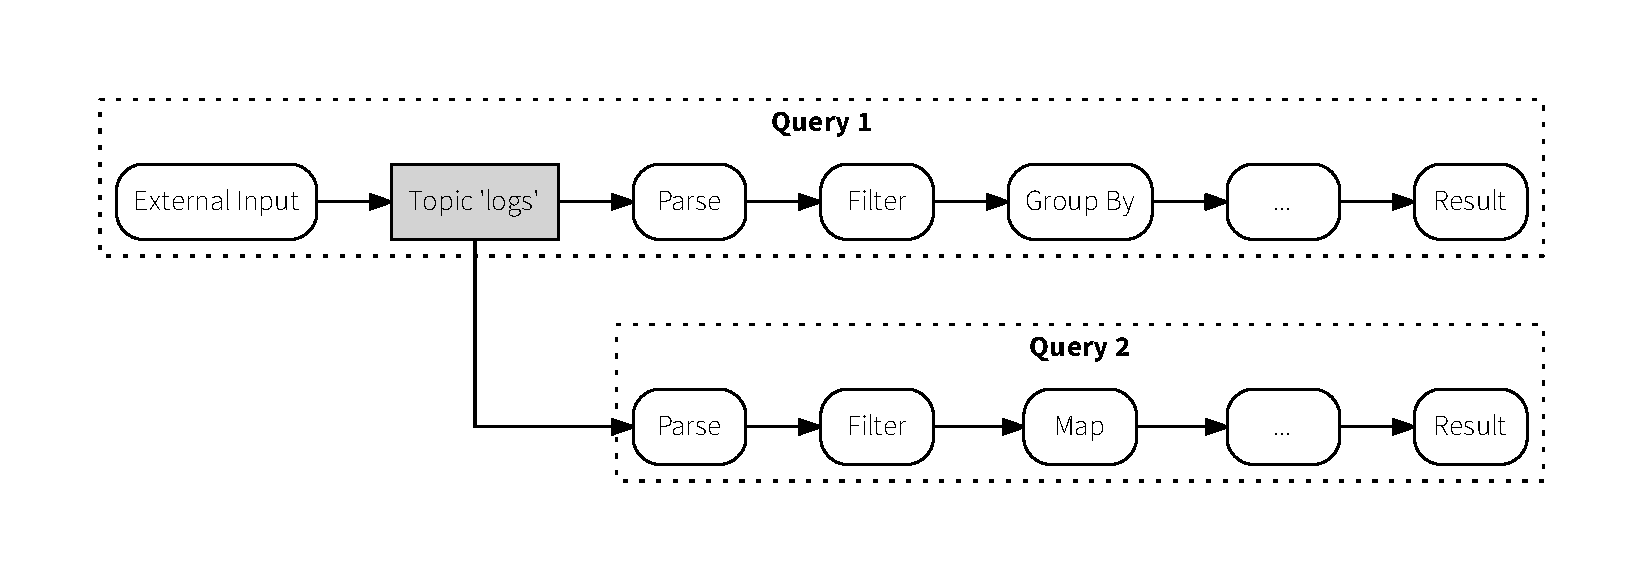
\includegraphics[scale=0.36]{figures/composition/q1q2_man}
  \vspace{-1.5em}
  \begin{center}
  $\Downarrow$
  \end{center}
  \vspace{-1.2em}
  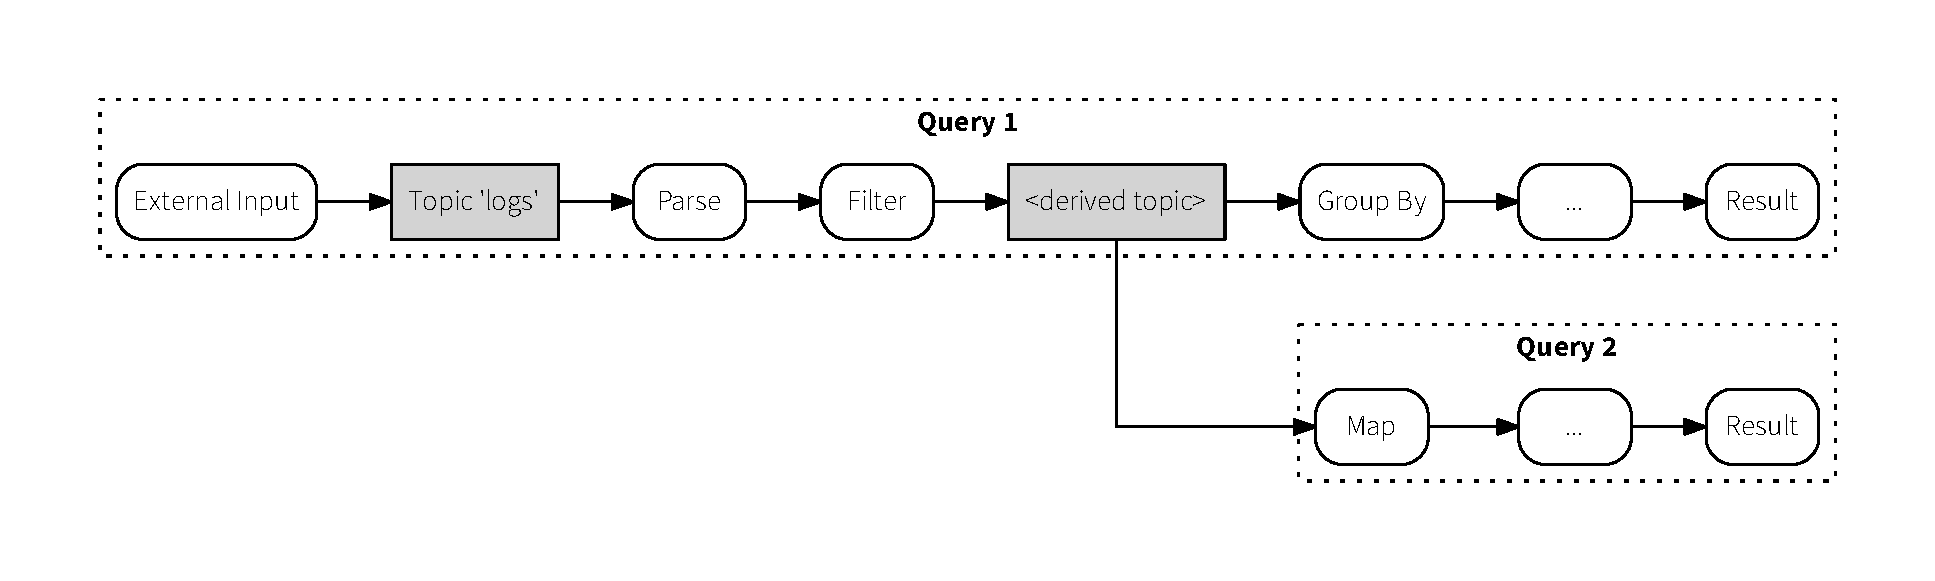
\includegraphics[scale=0.36]{figures/composition/q1q2_auto}
  \caption{Query optimization based on topic derivation. For identical
  operations on the same topic, the system would optimize the second
  query to avoid duplicated work.}
  \label{fig:queryoptimization}
\end{figure}




\subsection{Resource Management}

For the most part, resource management is still an unsolved problem in our
system: The placement of queries on executors is left to the submitting user.
While we believe that having this option is necessary: As discussed above, 
our system does not know much about the submitted queries, and thus does not
know what conditions have to be fulfilled for a good placement. In addition,
the submitting user might also always have external knowledge about the
available machines which is not expressed in the catalog.

However, in many cases automatic placement of queries is still desired. Future
work would have to explore what kind of information a query scheduler needs
from the executors to perform its task. In addition to monitoring, executors
could also control the resources allocated to a query, i.e. by using Linux
\emph{cgroups} \cite{cgroups} to ensure fair use of the available resources
by the running queries.

\subsection{Buffering and Backpressure}

If subscribers are connected, the publisher will buffer outgoing data for them
until the subscribers consume it or disconnect. This however can become an issue
if a single subscribers are slower than the publisher, as its queue grows and
memory consumption increases.

Our system allows that two queries subscribe from each other. Tightly coupled
queries thus can mitigate this problem by having the producer subscribe to
a \textquote{progress topic} published by the consumer. Future work could
explore more explicit mechanisms for notifying the publisher that it has to
slow down.

Another approach to deal with slow subscribers could be the introduction of
intermediate buffers close to the subscriber, a task typically done by the
message broker in other publish/subscribe systems. These buffers could
implement their own strategy how they want do deal with slow subscribers,
such as spilling to disk, or trying to restart slow subscribers with more
workers.

Intermediate buffers could be used to reduce network traffic, by having
multiple subscribers read their data from the local buffer instead remote
publishers.



\subsection{Persistence and Fault Tolerance}

\TODO{Timely Dataflow currently does not provide any means of fault tolerance. While
Naiad \cite{naiad} provided fault tolerance on the operator level, future work
could explore an implementation on the query level.}

\subsection{Partitioning and Filtering by Subscribers}

\TODO{In our current system, the partitioning scheme of published topics is
determined by the publishers. Kafka Streams and MillWheel both allow subscribers 
to provide partitioning functions which are used to decide how data is routed
from the publisher partitions to the subscriber instances.

This is also somewhat similar to content-based subscription.}

\clearpage
\section{Conclusions}

\cleardoublepage
%\addtocontents{toc}{\protect\clearpage} % <--- just debug stuff, ignore
%\include{multiToC} % <--- just debug stuff, ignore for your documents
% ********************************************************************
% Backmatter
%*******************************************************
\appendix
%\renewcommand{\thechapter}{\alph{chapter}}
\cleardoublepage
%\part{Appendix}
% TODO %********************************************************************
% Appendix
%*******************************************************
% If problems with the headers: get headings in appendix etc. right
%\markboth{\spacedlowsmallcaps{Appendix}}{\spacedlowsmallcaps{Appendix}}
\chapter{Appendix}
Lorem ipsum at nusquam appellantur his, ut eos erant homero
concludaturque. Albucius appellantur deterruisset id eam, vivendum
partiendo dissentiet ei ius. Vis melius facilisis ea, sea id convenire
referrentur, takimata adolescens ex duo. Ei harum argumentum per. Eam
vidit exerci appetere ad, ut vel zzril intellegam interpretaris.

%********************************************************************
% Other Stuff in the Back
%*******************************************************
\emergencystretch=1em
\cleardoublepage%********************************************************************
% Bibliography
%*******************************************************
% work-around to have small caps also here in the headline
\manualmark
\markboth{\spacedlowsmallcaps{\bibname}}{\spacedlowsmallcaps{\bibname}} % work-around to have small caps also
%\phantomsection 
\refstepcounter{dummy}
\addtocontents{toc}{\protect\vspace{\beforebibskip}} % to have the bib a bit from the rest in the toc
\addcontentsline{toc}{chapter}{\tocEntry{\bibname}}
\label{app:bibliography}
\printbibliography

\pdfbookmark[0]{Declaration of Originality}{declarationoforiginality}
% TODO 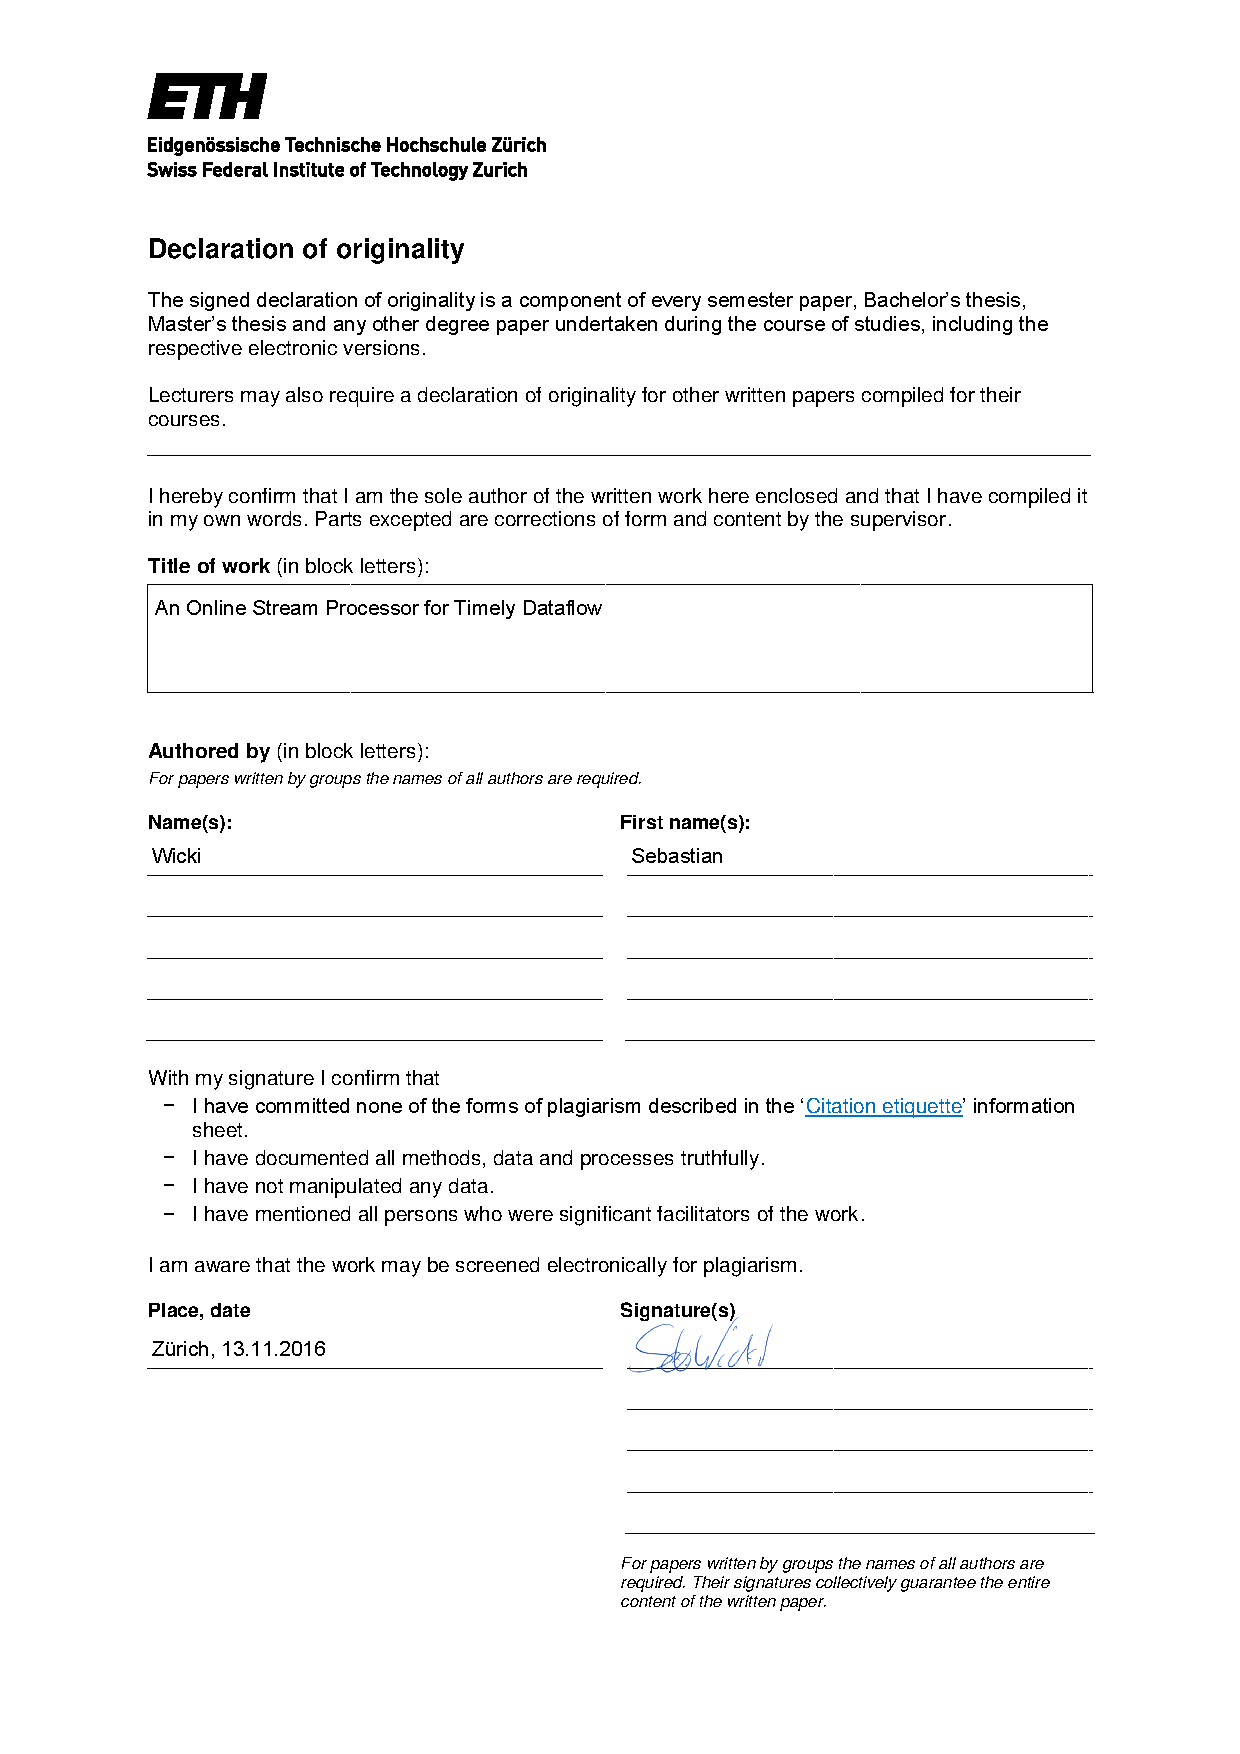
\includepdf[pages={1}]{frontback/declaration-originality.pdf}
% ********************************************************************
% Game Over: Restore, Restart, or Quit?
%*******************************************************
\end{document}
% ********************************************************************
